\documentclass[11pt]{article}
\usepackage[numbers]{natbib}
\usepackage{fullpage}
\usepackage{bm,amsmath,amsthm,amssymb,multicol,algorithmic,algorithm,enumitem}
\usepackage{wrapfig,lipsum}
\usepackage[textwidth=1cm,textsize=footnotesize]{todonotes}
\usepackage{caption}
% ready for submission
\usepackage{neurips_2020}
\usepackage{thm-restate}
\usepackage{comment}
\usepackage[colorlinks=true,
linkcolor=red,
urlcolor=blue,
citecolor=blue]{hyperref}
\usepackage{hyperref}
\usepackage{cleveref}
\usepackage{subfigure}
\usepackage{booktabs}
\setlength{\parskip}{.2cm}

 \makeatletter
\renewenvironment{proof}[1][\proofname]{%
   \par\pushQED{\qed}\normalfont%
   \topsep6\p@\@plus6\p@\relax
   \trivlist\item[\hskip\labelsep\bfseries#1]%
   \ignorespaces
}{%
   \popQED\endtrivlist\@endpefalse
}
\makeatother

%%%%%%%%%%% Stuffs for Tikz %%%%%%%%%%%%%%%%%%
\usepackage{pgfplots}
\usepackage{xargs}
\usepackage{stmaryrd}
\usetikzlibrary{arrows,shapes,calc,tikzmark,backgrounds,matrix,decorations.markings}
\usepgfplotslibrary{fillbetween}

\pgfplotsset{compat=1.3}

\usepackage{relsize}
\tikzset{fontscale/.style = {font=\relsize{#1}}
    }


%%%%%%%%%%%%%%%%%%%%%%%%%%%%%%%%%%%%%


\usepackage{shortcuts_OPT}

\makeatletter
\DeclareRobustCommand*\cal{\@fontswitch\relax\mathcal}
\makeatother

\begin{document}
\title{Towards Better Generalization of Adaptive Gradient Methods}
%\author{}
\date{\today}

\maketitle


\begin{abstract}
Adaptive gradient methods such as AdaGrad, RMSprop and Adam have been optimizers of choice for deep learning due to their fast training speed. However, it was recently observed that their generalization performance is often worse than that of SGD for over-parameterized neural networks. While new algorithms such as AdaBound, SWAT, and Padam were proposed to improve the situation, the provided analyses are only committed to optimization bounds with training, leaving critical generalization capacity unexplored. To close this gap, we propose \textit{\textbf{S}table \textbf{A}daptive \textbf{G}radient \textbf{D}escent} (\textsc{SAGD}) for non-convex optimization which leverages differential privacy to boost the generalization performance of adaptive gradient methods. Theoretical analyses show that \textsc{SAGD} has high-probability convergence to a population stationary point. We further conduct experiments on various popular deep learning tasks and models. Experimental results illustrate that \textsc{SAGD} is empirically competitive and often better than baselines. 
\end{abstract}

\section{Introduction}

We consider in this paper, the following minimization problem:
\begin{equation} \label{eq: problem}
 \min_{\w \in \cW}~ f({\w})  \triangleq {\mathbb{E}_{z \sim \mathcal{P}}}[\ell(\w,z)]~,
\end{equation}
where the \emph{population loss} $f$ is a (possibly) nonconvex objective function (as for most deep learning tasks), $\cW \subset \R^d$ is the parameter set and $z$ is the vector of data samples distributed according to an unknown data distribution $\mathcal{P}$. 
We assume that we have access to an oracle that, given $n $ i.i.d. samples $(\z_{1}, \dots, \z_{n})$, returns the stochastic objectives $(\ell(\w,\z_{1}), \dots, \ell(\w,\z_{n}))$.
Our goal is to find critical points of the population loss function.
Given the unknown data distribution, a natural approach towards solving \eqref{eq: problem} is empirical risk minimization (ERM)~\citep{shbe14}, which minimizes the \emph{empirical loss} $\hat f(\w)$ as follows: $\min_{\w \in \cW}     \hat f(\w)  \triangleq \frac{1}{n}\sum_{j =1}^{n} \ell(\w, \z_j)$, when $n$ samples $\z_{1}, \dots, \z_{n}$ are observed.
Stochastic gradient descent (SGD)~\citep{romo51} which iteratively updates the parameter of a model by descending along the negative gradient computed on a single sample or a mini-batch of samples has been most dominant algorithms for solving the ERM problem, e.g., training deep neural networks. To automatically tune the learning-rate decay in SGD, adaptive gradient methods, such as AdaGrad~\citep{duha11}, RMSprop~\citep{tige12}, and Adam~\citep{kiba15}, have emerged leveraging adaptive coordinate-wise learning rates for faster convergence.

However, the generalization ability of these adaptive methods is often worse than that of SGD for over-parameterized neural networks, e.g., convolutional neural network (CNN) for image classification and recurrent neural network (RNN) for language modeling~\citep{wiro17}. 
To mitigate this issue, several recent algorithms were proposed to combine adaptive methods with SGD.
For example, AdaBound~\citep{luxi2019} and SWAT~\citep{keso2017} switch from Adam to SGD as the training proceeds, while Padam~\citep{chgu2018, zhta18} unifies AMSGrad~\citep{reka2018} and SGD with a partially adaptive parameter.  
Despite much efforts on deriving theoretical convergence results of the objective function \citep{zare18,wawu19, zosh2019, cheli2019}, these newly proposed adaptive gradient methods are often misunderstood regarding their generalization capacity, which is the ultimate goal.
On the other hand, current adaptive gradient methods~\citep{duha11,kiba15,tige12, reka2018, wawu19} follow a typical stochastic optimization (SO) oracle~\citep{romo51, ghla2013} which uses stochastic gradients to update the parameter. The SO oracle requires \emph{new samples} at every iteration to get the stochastic gradient such that it equals the population gradient in expectation. In practice, however, only finite training samples are available and reused by the optimization oracle for a certain number of times (a.k.a., epochs). 
~\citet{hare2016} found that the generalization error increases with the number of times the optimization oracle passes the training data. 
It is thus expected that gradient descent algorithms will be much more well-behaved if we have access to infinite fresh samples. 
Re-using data samples is therefore a caveat for the generalization of a given algorithm.

In order to tackle the above issues, we propose \textit{\textbf{S}table \textbf{A}daptive \textbf{G}radient \textbf{D}escent} (\textsc{SAGD}) which aims at improving the generalization of general adaptive gradient descent algorithms.
\textsc{SAGD} behaves similarly to the aforementioned ideal case of infinite fresh samples borrowing ideas from \emph{adaptive data analysis}~\citep{dwfe15} and \emph{differential privacy}~\citep{dwro2014}. 
The main idea of our method is that, at each iteration, \textsc{SAGD} accesses the training set $z$ through a differentially private mechanism and computes an estimated gradient $\nabla \ell(\w,z)$ of the objective function $\nabla f(\w)$. 
It then uses the estimated gradient to perform a descent step using adaptive step size. 
We prove that the reused data points in \textsc{SAGD} nearly possesses the statistical nature of \emph{fresh samples} yielding to high concentration bounds of the population gradients through the iterations.

Our  contributions  can be summarized as follows:
\begin{itemize}
\item We derive a novel adaptive gradient method, namely \textsc{SAGD}, leveraging ideas of differential privacy and adaptive data analysis aiming at improving the generalization of current baseline methods. A mini-batch variant is also introduced for large-scale learning tasks.
\item Our differentially private mechanism, embedded in the \textsc{SAGD}, explores the idea of Laplace Mechanism (adding Laplace noises to gradients) and Thresholdout~\citep{dwro2014} leading to DPG-Lap and DPG-Sparse methods which potentially saves privacy cost. In particular, we show that differentially private gradients stay close to the population gradients with high probability. 
\item We establish various theoretical guarantees for our algorithm. We first show that the $\ell_2$-norm of the \emph{population gradient}, i.e., $\|\nabla f(\w)\|$ obtained by the \textsc{SAGD} converges with high probability. Then, we present a generalization analysis of the proposed algorithms, showing that the norm of the population gradient converges with high probability.
\item We conduct several experimental applications based on training neural networks for image classification and language modeling indicating that \textsc{SAGD} outperforms existing adaptive gradient methods in terms of the generalization performance.
\end{itemize}
The remainder of the paper is organized as follows.
Section~\ref{related} describes related work and notations. 
The \textsc{SAGD} algorithm, including the differentially private mechanisms, and its mini-batch variant are described in Section~\ref{algorithm}. 
Numerical experiments are presented Section~\ref{sec: experiment}. 
Section~\ref{sec: conclusion} concludes our work. 
Due to space limit, most of the proofs are deferred to the supplementary material.

\textbf{Related work:}
%{\bf Adaptive Gradient Methods:} 
%Adaptive gradient methods usually refer to a class of algorithms that change learning rates adaptively during optimization. Alone this line, many variants have been proposed, including AdaGrad~\citep{duha11}, RMSprop~\citep{tige12}, and Adam~\citep{kiba15}, and AMSGrad~\citep{sare18}, which use the second moment of gradients to change the learning rates on different coordinates to adapt to the geometry of the loss function. 
In the non-convex setting, existing work on SGD~\citep{ghla2013} and adaptive gradient methods~\citep{zare18, wawu19, zosh2019, cheli2019} 
shows convergence to a stationary point with a rate of  $O(1/\sqrt{T})$
where $T$ is the number of stochastic gradient computations. Given $n$ samples, a stochastic oracle can obtain at most $n$ stochastic gradients
, which implies convergence to the population stationarity with a rate of $O(1/\sqrt{n})$.
%generalization bound.
%(the norm of the population gradient converges as $\|\nabla f(\w)\| \leq O(1/\sqrt{n}$),i .e., $O(1/\sqrt{n})$. 
In addition, ~\citet{kula2018, rara2017, hare2016,mowa2018, pejo2018, cheli2019, lilu2019} studied 
the generalization of gradient-based optimization algorithms using the generalization property of algorithm stability~\cite{boel02}. Particularly,~\citet{rara2017, mowa2018, lilu2019, pejo2018} focus on noisy gradient algorithms, e.g., SGLD, and provide a generalization error (population risk minus empirical risk) bound as $O(\sqrt{T}/n)$. This type of bounds usually has a dependence on the training data and has polynomial dependence on the iteration number $T$.  This work focuses on the first type of bounds, i.e., the $\ell_2$-norm of the gradient.

%\noindent{\bf Differential Privacy and Adaptive Data Analysis:} 
Differential privacy~\cite{dwro2014} was originally studied for preserving the privacy of individual data in the statistical query. Recently, differential privacy has been widely used in the area of optimization. Some pioneering work~\citep{chmo2011, basm2014, waye2017} introduced differential privacy to empirical risk minimization (ERM) to protect sensitive information of the training data. The popular differentially private
algorithms includes the gradient perturbation that adds noise to the gradient in gradient descent algorithms~\citep{chmo2011,basm2014,waxu2019}.
%There are some differentially private
%algorithms, such as output-perturbation that perturbs the output of a non-DP algorithm, objective function perturbation that perturbs the objective function~\citep{chmo2011} and gradient perturbation that adds noise to the gradient in gradient descent algorithms~\citep{basm2014} have been proposed.~\citet{waxu2019} studied differential private gradient descent algorithms for non-convex empirical risk minimization. 
Actually, except for preserving the privacy, differential privacy also has the property of guarantee generalization in adaptive data analysis (ADA) ~\cite{dwfe2015a,dwfe2015b,dwfe2015c}. In ADA, a holdout set is reused for multiple times to test the hypotheses which are generated based previous test result.  It has been shown that reusing the holdout set via a differentially private mechanism ensures the validity of the test. In other words, the differentially private reused dataset maintains the statistical nature of fresh samples. 
\citet{dwfe2015a, dwfe2015b, dwfe2015c} designed a practical method named Thresholdout, which can be used to test a large number of hypotheses. 
\citet{zhch2018} extended the idea of differential privacy and adaptive data analysis to convex optimization and provides generalization error bound.
%However, none of these methods uses adaptive step size and one has to manually tune the learning rate as the training proceeds.

\textbf{Notations} 
We use $\g_t$ and $\nabla f(\w)$ interchangeably to denote the \emph{population gradient} such that $\g_t = \nabla f(\w_t) = \mathbb{E}_{\z \in \cP} [\nabla \ell(\w_t, \z)]$. $S = \left\{\z_{1}, \dots, \z_{n}\right\}$
denotes the $n$ available training samples. $\hat \g_t$ denotes the sample gradient evaluated on $S$ such that $\hat \g_t = \nabla \hat f(\w) = \frac{1}{n}\sum_{j=1}^n \nabla \ell(\w_t, \z_j)$. For a vector $\v$, $\v^2$ represents that $\v$ is element-wise squared.  We use $\v^i$ or $[\v]_i$ to denote the $i$-th coordinate of $\v$ and $\|\v\|_2$ is the $\ell_2$-norm of $\v$.
\begin{defn}
(Differential Privacy~\citep{dwro2014}) A randomized algorithm $\mathcal{M}$ is $(\epsilon, \delta)$-differentially private if 
    \[
    \mathbb{P}\{\mathcal{M}(\cal{D})\in \mathcal{Y}\} \leq \exp(\epsilon)\mathbb{P}\{\mathcal{M}(\cal{D\prime})\in \mathcal{Y} \} + \delta.
    \]
holds for all $\mathcal{Y}\subseteq Range(\mathcal{M})$ and all pairs of adjacent datasets $\cal{D},\cal{D\prime}$ that differ on a single sample.
\end{defn}
%Intuitively, differential privacy means that the outcomes of two nearly identical  datasets should be nearly identical such that an analyst will not be able to distinguish any single data point by monitoring the change of the output. 
%In the context of machine learning, this randomized algorithm $\mathcal{M}$ could be a learning algorithm that outputs a classifier, i.e., $\mathcal{M}(D)=f$, where $D$ is the training set. For gradient-based optimization algorithms, $\mathcal{M}$ could be a gradient computing method that outputs an estimated gradient, i.e., $\mathcal{M}(D)=\g$. 
The general approach for achieving  $(\epsilon, \delta)$-differential privacy when estimating a deterministic real-valued function $q: \cZ^n \rightarrow \mathbb{R}^d$ is Laplace Mechanism~\citep{dwro2014}, which adds Laplace noise calibrated to the function $q$, i.e., $\mathcal{M}(\cD)= q(\cD)+ \b$, where $\b^i, \forall i \in [d]$ is drawn from a Laplace Distribution with variance $\sigma^2$ and zero mean.

\section{Stable Adaptive Gradient Descent Algorithm}
\label{algorithm}

In this section, we present \textsc{SAGD} with two differentially private methods to compute the estimated gradient, namely DPG-Lap and DPG-Sparse.
We present the \textsc{SAGD} algorithm in two parts: adaptive gradient for updating the parameter (Algorithm~\ref{algo: StAda}), and \textbf{D}ifferential \textbf{P}rivate\textbf{ G}radient (DPG, Algorithm~\ref{algo: lap}) for updating the gradient. Algorithm~\ref{algo: StAda} uses 
DPG to obtain an estimated gradient (line 4 in Algorithm~\ref{algo: StAda}). For DPG, we first provide a basic algorithm named \emph{DPG-Lap} which is based on the \emph{Laplace Mechanism}~\citep{dwro2014} in Section~\ref{subsec: SAGD_lap}. Later on, we provide an advanced version named \emph{DPG-Sparse} which is motivated by sparse vector technique~\citep{dwro2014} in Section~\ref{subsec: SAGD-sparse}.


\subsection{\textsc{SAGD} with DPG-LAP} \label{subsec: SAGD_lap}

We provide the pseudo code of \textsc{SAGD} in Algorithm~\ref{algo: StAda}. 
Given $n$ training samples $S$, loss function $\ell$, at each iteration $t \in [T]$, Algorithm~\ref{algo: StAda} calls DPG($S$,  $\ell(\cdot)$, $\w_t$, $\sigma$) to access the training set $S$ and obtain an estimate $\tilde \g_t$ (line 4), then updates $\w_{t+1}$ based on $\tilde \g_1,..., \tilde \g_t$ using the adaptive step size (line 5, 6):
$\m_t = \tilde \g_t$, $\v_t = \left(1-\beta_{2}\right) \sum_{i=1}^{t} \beta_{2}^{t-i} \tilde \g_{i}^{2}$, and $\w_{t+1}=\w_{t}-\eta_t \m_t /(\sqrt{\v_t}+\nu)$.
Note that noise variance $\sigma^2$, step-size $\eta_t$, and iteration number $T$, $~ \beta_2,~\nu$ are the parameters of Algorithm~\ref{algo: StAda}. 
We analyze the optimal values of them for \textsc{SAGD} in the subsequent sections. 

\begin{algorithm}[H] 
\caption{\textsc{SAGD}}
\begin{algorithmic}[1] \label{algo: StAda}
\STATE \textbf{Input}: Dataset $S$,  certain loss $\ell(\cdot)$, initial point $\w_0$.
\STATE Set  noise level $\sigma$, iteration number $T$,  and step size $\eta_t$.
\FOR{$t = 0,...,T-1$}
\STATE  Call DPG($S$,  $\ell(\cdot)$, $\w_t$, $\sigma$) to compute gradient $\tilde \g_t$.
\STATE 
$\m_t = \tilde \g_t$ and $\v_t = \left(1-\beta_{2}\right) \sum_{i=1}^{t} \beta_{2}^{t-i} \tilde \g_{i}^{2}$.
\STATE $\w_{t+1}=\w_{t}-\eta_t \m_t /(\sqrt{\v_t}+\nu)$.
\ENDFOR 
\end{algorithmic}
\end{algorithm}

For the DPG, we first consider \emph{DPG-Lap} (Algorithm~\ref{algo: lap}) which adds Laplace noises $\b_t \in \mathbb{R}^d$ to the empirical gradient $\hat \g_t = \frac{1}{n} \sum_{j=1}^n\nabla \ell(\w_t, \z_j)$ and returns a noisy gradient $\tilde \g_t = \hat \g_t + \b_t$ to the optimization oracle Algorithm~\ref{algo: StAda}. 

\begin{algorithm}[H]
\caption{DPG-Lap}
\begin{algorithmic}[1]
\label{algo: lap}
	\STATE \textbf{Input}: Dataset $S$,  certain loss $\ell(\cdot)$, parameter $\w_t$, noise level $\sigma$.
	\STATE Compute full batch gradient on $S$: \\
	\centerline{ $\hat \g_t = \frac{1}{n} \sum_{j=1}^n\nabla \ell(\w_t, z_j)$.}	
	\STATE Set $\tilde \g_t = \hat \g_t + \b_t$, where $\b_t^i$ is drawn i.i.d from Lap$(\sigma), \forall\, i \in [d]$.
	\STATE \textbf{Output}: $\tilde \g_t$.
	\end{algorithmic}
\end{algorithm}

In the sequel, the following assumptions are necessary:
\begin{assumption}
The objective function $ f: \mathbb{R}^d \rightarrow \mathbb{R}$ is bounded from below by $f^\star$ and is $L$-smooth ($L$-Lipschitz gradients), i.e.,$\nr \|\nabla f(\w) -\nabla f(\w^\prime) \|\leq L \|\w-\w^\prime \|, ~ \forall\, \w, \w^\prime \in \cW$.
\end{assumption}
\begin{assumption}
The gradient of $f$ and its noisy approximation are bounded: $\|\nabla \ell (\w, z) \|_1 \leq G_1, \ \forall\,\w \in \cW, \  \z \in \cZ$ and $\|\tilde \g_t\|_2 \leq G, \forall t \in [T]$.
\end{assumption}
To analyze the convergence of \textsc{SAGD} in terms of $\ell_2$ norm of the population gradient, we need to 
show that $\tilde \g_t$ approximate the population gradient $\g_t$ with high probability, i.e., the estimation error $\| \tilde \g_t - \g_t\|$ is small at every iteration.  To make such an analysis, we first present the generalization guarantee of any differentially private algorithm in Lemma~\ref{lem: gen_adv}, then we show that \textsc{SAGD} is differentially private in Lemma~\ref{lemma dpp}. It is followed by establishing \textsc{SAGD}'s generalization guarantee in Theorem~\ref{thm: acc_basic}, i.e., estimated $\tilde \g_t$ approximates the population gradient $\g_t$ with high probability. Last, we prove that \textsc{SAGD} converges to a population stationary point with high probability in Theorem~\ref{thm: main_rmsprop}.


The general approach for analyzing the estimation error of sample gradient to population gradient is the Hoeffding’s bound. 
Given training set $S \in \mathcal{Z}^n$ and a fixed $\w_0$ chosen to be independent of the dataset $S$,  we have empirical gradient $\hat \g_0= \mathbb{E}_{z \in S}\nabla \ell(\w_0,z)$ and population gradient $\g_0 = \mathbb{E}_{z\sim \mathcal{P}}[\nabla l(\w_0,z)]$. Hoeffding’s bound implies generalization of fresh samples, i.e., for every coordinate $i \in [d]$ and $\mu > 0$,  empirical gradients are concentrated around population gradients, i.e., 
	\begin{equation} \label{hoeffding}
	P\{|\hat \g^i_0 - \g_0^i | \geq \mu \} \leq2 \exp \left(\frac{-2n\mu^2}{4G_\infty^2} \right),
	%	P \{ | \hat g_i(w_0) - g_i(w_0) | \geqslant \sigma \} \leqslant 2 \exp \left(\frac{-2n\sigma^2}{4 G^2}\right),
	\end{equation}
 where $G_\infty$ is the maximal value of the $\ell_\infty$-norm of the gradient $ \g_0$. Generally, if $\w_1$ is updated using the gradient computed on training set $S$, i.e., $\w_1 = \w_0 - \eta \hat \g_0$, the above concentration inequality \emph{will not} hold for $\hat \g_1 = \mathbb{E}_{z \in S}\nabla_i \ell(\w_1,z)$, because $\w_1$ is no longer independent of dataset $S$. However, Lemma~\ref{lem: gen_adv} shows that if $\w_t, \forall\, t \in [T]$ is generated by reusing $S$ under a differentially private mechanism, concentration bounds similar to Eq.~(\ref{hoeffding}) will hold for all $\w_1, \w_2,...,\w_T$ that are adaptively generated on the same dataset $S$. 

\begin{restatable}{lemm}{lemgenadv}
\label{lem: gen_adv}
	Let $\cA$ be an $(\epsilon, \delta)$-differentially private gradient descent algorithm with access to training set $S$ of size $n$. Let $\w_t = \cA(S)$ be the parameter generated at iteration $t \in [T]$ and $\hat \g_t$ the empirical gradient on $S$. For any $\sigma >0$, $\beta > 0$, if the privacy cost of $\cA$ satisfies $\epsilon \leq \frac{\sigma}{13}$, $\delta \leq \frac{\sigma \beta}{26 \ln(26/\sigma)}$, and sample size $n \geq \frac{2\ln(8/\delta)}{\epsilon^2}$, we then have
	\begin{equation*}
	\mathbb{P}\left\{ |\hat \g_t^i - \g_t^i| \geq  \sigma \right\} \leq \beta \quad \textrm{for every $ i\in [d]$ and every $t \in [T]$} .
	\end{equation*} 
\end{restatable}
Lemma~\ref{lem: gen_adv} is an instance of Theorem 8 from~\cite{dwfe15} and illustrates, if the privacy cost $\epsilon$ is bounded by the estimation error, that differential privacy enables the reused training set to maintain statistical guarantees as a fresh sample. Next, we analyze the privacy cost of \textsc{SAGD} in Lemma~\ref{lemma dpp}.



\begin{restatable}{lemm}{lemdpp}
\label{lemma dpp}
	\textsc{SAGD} with DPG-Lap is 
	$(\frac{\sqrt{T \ln(1/\delta)} G_1}{n\sigma}, \delta)$-differentially private. 
\end{restatable} 


In order to achieve a gradient concentration bound for \textsc{SAGD} with DPG-Lap as described in Lemma~\ref{lem: gen_adv}, we need to set $\frac{\sqrt{T \ln(1/\delta)} G_1}{n\sigma} \leq \frac{\sigma}{13}$, $\delta \leq \frac{\sigma \beta}{26 \ln(26/\sigma)}$, and  sample size $n \geq \frac{2\ln(8/\delta)}{\epsilon^2}$. We then have the following theorem showing that across all iterations, gradients produced by \textsc{SAGD} with DPG-Lap maintain high probability concentration bounds.

\begin{restatable}{theo}{theoaccbasic}
\label{thm: acc_basic}
Given parameter $\sigma > 0$, let $\tilde \g_1,...,  \tilde \g_T$ be the gradients computed by DPG-Lap in \textsc{SAGD} over $T$ iterations. Set the total number of iterations $ \frac{2n\sigma^2}{G_1^2}\leq T \leq \frac{n^2 \sigma^4}{169 \ln(1/(\sigma \beta))G_1^2}$, then for $\forall\, t \in [T]$ any $\beta >0$, and any $\mu > 0$ we have:
    \begin{equation*}
    \mathbb{P}\left\{\|\tilde \g_t - \g_t\| \geq \sqrt{d}\sigma(1+\mu)\right\} \leq d\beta + d\exp(-\mu).
    \end{equation*}
\end{restatable}


Theorem~\ref{thm: acc_basic} indicates that gradient $\tilde \g_t$
produced by DPG-Lap is concentrated around population gradient $\g_t$ with a tight concentration error bound $\sqrt{d}\sigma(1+\mu)$. A higher noise level $\sigma$ brings a better privacy 
guarantee  and a larger number of iterations $T$, but meanwhile incurs a 
larger concentration error $\sqrt{d}\sigma(1+\mu)$. Thus, there is a trade-off between noise and accuracy. $\beta$ and $\mu$ are any positive numbers that illustrate the trade-off between the concentration error and the probability. A larger $\mu$ brings a larger concentration error but a smaller probability. For $\beta$, if we increase $\beta$, we get a larger upper bound on $T$, which means the concentration bound will hold for more iterations, but we also get a larger probability. Note that although the probability $d\beta + d\exp(-\mu)$ has a dependence on dimension $d$, we can choose appropriate $\beta$ and $\mu$ to make the probability arbitrarily small.  We optimize the choice of $\beta$ and $\mu$ when analyzing the convergence to the population stationary point.

We derive the optimal values of $\sigma$ and $T$ to optimize the trade-off between statistical rate and optimization rate and obtain the optimal bound in Theorem~\ref{thm: main_rmsprop}. For brevity, let $\rho_{n,d} \triangleq O \left(\ln n + \ln d\right)$.


\begin{restatable}{theo}{theomainrmsprop}
\label{thm: main_rmsprop}
 Given training set $S$ of size $n$, for $\nu >0$, if $\eta_t = \eta$ which are chosen with $\eta \leq \frac{\nu}{2L}$,  $\sigma = 1/n^{1/3}$, and iteration number $T = n^{2/3}/\left(169G_1^2(\ln d + \frac{7}{3}\ln n)\right)$, then \textsc{SAGD} with DPG-Lap converges to a stationary point of the population risk, i.e., 
 \begin{small}
\begin{equation*}
 \min_{1\leq t \leq T}\|\nabla f(\w_t)\|^2 \leq
 O \left( \frac{\rho_{n,d} \left(f(\w_1) - f^\star \right)}{n^{2/3}} \right) + O \left( \frac{d \rho_{n,d}^2}{n^{2/3}}\right),
\end{equation*}
\end{small}
with probability at least $1-O\left(\frac{1}{\rho_{n,d} n}\right)$.
\end{restatable} 


Theorem~\ref{thm: main_rmsprop} shows that, given $n$ samples, \textsc{SAGD} converges to a population stationary point at a rate of $O(1/n^{2/3})$. Particularly, the first term of the bound corresponds to the optimization error $O(1/T)$ with $T = O(n^{2/3})$, while the second is the statistical error depending on available sample size $n$ and dimension $d$. In terms of computation complexity, \textsc{SAGD} 
requires $O(n^{5/2})$ stochastic gradient computations for $O(n^{3/2})$ passes over $n$ samples. The current optimization analyses~\citep{zare18, wawu19, zosh2019, cheli2019} show that 
adaptive gradient descent algorithms (SO oracle) converges to the population stationary point with a rate of $O(1/\sqrt{T})$ with $T$ stochastic gradient computations. Given $n$ samples, their analyses give a rate of  $O(1/\sqrt{n})$. The \textsc{SAGD} achieves a sharper bound compared to the previous analyses.  
We will consider improving the dependence on dimension $d$ in our future work.



\vspace{-0.05in}
\subsection{\textsc{SAGD} with DPG-SPARSE} \label{subsec: SAGD-sparse}

In this section, we consider the \textsc{SAGD} with an advanced version of DPG named \emph{DPG-Sparse} which is motivated by sparse vector technique~\citep{dwro2014} aiming to provide a sharper result on the privacy cost $\epsilon$ and $\delta$.

Lemma~\ref{lemma dpp} shows that the privacy cost of \textsc{SAGD} with DPG-Lap scales with $O(\sqrt{T})$. In order to guarantee the generalization of \textsc{SAGD} as stated in Theorem~\ref{thm: acc_basic}, we need to control the privacy cost below a certain threshold i.e., $\frac{\sqrt{T \ln(1/\delta)} G_1}{n\sigma} \leq \frac{\sigma}{13}$. However, it limits the iteration number $T$ of \textsc{SAGD}, leading to a compromised optimization term in Theorem~\ref{thm: main_rmsprop}.  To achieve relax the upper bound on the $T$, we use another differentially private
mechanism, i.e., sparse vector technique~\citep{dwfe15,dwfe2015b,dwfe2015c,dwro2014} instead of Laplace Mechanism to reduce the privacy cost. Thus, we propose an alternative to DPG, named \textsc{SAGD} with DPG-Sparse (Algorithm~\ref{algo: sparse}).


Given $n$ samples, Algorithm~\ref{algo: sparse} splits the dataset evenly into two parts $S_1$ and $S_2$. At every iteration $t$, Algorithm~\ref{algo: sparse}  computes gradients on both datasets:
$\hat \g_{S_1,t} = \frac{1}{|S_1|} \sum_{\z_j \in S_1}\nabla \ell(\w_t, \z_j)$ and $\hat \g_{S_2,t} = \frac{1}{|S_2|} \sum_{\z_j \in S_2}\nabla \ell(\w_t, \z_j)$.
%\begin{eqnarray*}
%\hat \g_{S_1,t} &=& \frac{1}{|S_1|} \sum_{\z_j \in S_1}\nabla \ell(\w_t, \z_j),\\
%\hat \g_{S_2,t} &=& \frac{1}{|S_2|} \sum_{\z_j \in S_2}\nabla \ell(\w_t, \z_j).
%\end{eqnarray*}
It then validates $\hat \g_{S_1,t} $ with $\hat \g_{S_2,t}$. That is, if the norm of their difference is greater than a random threshold $\tau-\gamma$, it then returns $\tilde \g_t = \hat \g_{S_1,t} + \b_t$, otherwise $\tilde \g_t = \hat \g_{S_2,t}$. 
Note that Algorithm~\ref{algo: sparse} is an extension of Thresholdout in~\citet{zhch2018}.
Inspired by Thresholdout,~\citet{zhch2018} proposed stable gradient descent algorithms which use a similar framework as DPG-Sparse to compute an estimated gradient by validating each coordinate of $\hat \g_{S_1,t}$ and $\hat \g_{S_2,t}$. However, their  method is computationally expensive in high-dimensional settings such as deep neural networks. 

%DPG-Sparse is an advanced method of differential privacy mechanism which saves privacy cost. We will explain in the following parts. 

%\yz{have to compare with zhou et al 2018}

\begin{algorithm}[H]
\caption{\textsc{SAGD} with DPG-Sparse}
\begin{algorithmic}[1]
\label{algo: sparse}
\STATE \textbf{Input}: Dataset $S$,  certain loss $\ell(\cdot)$, initial point $\w_0$.
%sequence of functions $\{\phi_t, \psi_t \}_{t=0}^{T-1}$
\STATE Set  noise level $\sigma$, iteration number $T$,  and step size $\eta_t$.
\STATE Split $S$ randomly into $S_1$ and $S_2$. 
\FOR{$t = 0,...,T-1$}
\STATE   Compute full batch gradient on $S_1$ and $S_2$:\\
\centerline{$\hat \g_{S_1,t} = \frac{1}{|S_1|} \sum_{\z_j \in S_1}\nabla \ell(\w_t, \z_j)$,}
\centerline{$\hat \g_{S_2,t} = \frac{1}{|S_2|} \sum_{\z_j \in S_2}\nabla \ell(\w_t, \z_j)$.}
\STATE Sample $\gamma \sim \text{Lap}(2\sigma)$, $\tau \sim \text{Lap}(4\sigma)$.
\IF{$\| \hat \g_{S_1,t} - \hat \g_{S_2,t}\| + \gamma >  \tau$}
\STATE  $\tilde \g_t = \hat \g_{S_1,t} + \b_t$, where $\b_t^i$ is drawn i.i.d from Lap$(\sigma), \forall\, i \in [d]$.
\ELSE \STATE $\tilde \g_t = \hat \g_{S_2,t}$
\ENDIF
\STATE 
$\m_t = \tilde \g_t$ and $\v_t = \left(1-\beta_{2}\right) \sum_{i=1}^{t} \beta_{2}^{t-i} \tilde \g_{i}^{2}$.
%$\m_t = \phi_t(\tilde \g_1, ..., \tilde \g_t)$ and $\v_t = \psi_t(\tilde \g_1,.., \tilde \g_t)$
\STATE $\w_{t+1}=\w_{t}-\eta_t \m_t /(\sqrt{\v_t}+\nu)$.
\ENDFOR 
\STATE \textbf{Return}: $\tilde \g_t$.
\end{algorithmic}
\end{algorithm}


To analyze the privacy cost of DPG-Sparse, let $C_{s}$ be the number of times the validation fails, i.e., $\| \hat \g_{S_1,t} - \hat \g_{S_2,t}\| + \gamma >  \tau$ is true, over $T$ iterations in \textsc{SAGD}. The following Lemma presents the privacy cost of \textsc{SAGD} with DPG-Sparse.

\begin{restatable}{lemm}{lemdppsparse}
\label{lemma: dpp-sparse}
\textsc{SAGD} with DPG-Sparse  (Algorithm 3) is  
$(\frac{\sqrt{C_{s} \ln(2/\delta)} 2G_1}{n\sigma}, \delta)$-differentially private. 
\end{restatable}




Lemma~\ref{lemma: dpp-sparse} shows that the privacy cost of  \textsc{SAGD} with DPG-Sparse scales with $O(\sqrt{C_{s}})$ where $C_{s} \leq T$. In other words, DPG-Sparse saves the privacy cost of \textsc{SAGD}. In order to achieve the generalization guarantee of \textsc{SAGD} with DPG-Sparse as stated in Lemma~\ref{lem: gen_adv},  by considering the guarantee of Lemma~\ref{lemma: dpp-sparse},  we only need to set $\frac{\sqrt{C_{s} \ln(1/\delta)} G_1}{n\sigma} \leq \frac{\sigma}{13}$, which potentially improves the upper bound of $T$. 
%$\delta \leq \frac{\sigma \beta}{26 \ln(26/\sigma)}$, and sample size $n \geq \frac{2\ln(8/\delta)}{\epsilon^2}$.  
The following theorem shows the generalization guarantee of $\tilde \g_t$ generated by \textsc{SAGD} with DPG-Sparse.

\begin{restatable}{theo}{theoaccsparse}
\label{thm: acc_sparse}
Given parameter $\sigma > 0$, let $\tilde \g_1,...,  \tilde \g_T$ be the gradients computed by DPG-Sparse over $T$ iterations. With a budget $ \frac{n\sigma^2}{2G_1^2} \leq C_{s} \leq\frac{n^2 \sigma^4}{676 \ln(1/(\sigma \beta))G_1^2}$, for $\forall\, t \in [T]$, any $\beta > 0$, and any $\mu > 0$ we have 
        \begin{equation*}
    \mathbb{P}\left\{\|\tilde \g_t - \g_t\| \geq \sqrt{d}\sigma(1+\mu)\right\} \leq d\beta + d\exp(-\mu).
    \end{equation*}
\end{restatable}

%Note that $C_{s}$ is much smaller than $T$ which 

In the worst case $C_{s} = T$, we can recover the upper bound of $T$ as $T \leq \frac{n^2 \sigma^4}{676 \ln(1/(\sigma \beta))G_1^2}$. DPG-Sparse behaves as DPG-Lap in this worst case.
The following theorem displays the \emph{worst case bound} of \textsc{SAGD} with DPG-Sparse.
%Next we consider \textsc{SAGD} with updating rule of RMSprop: $\phi_t(\tilde \g_1,...,\tilde \g_t) = \tilde \g_t$ and $ \v_t = \left(1-\beta_{2}\right) \sum_{i=1}^{t} \beta_{2}^{t-i} \tilde \g_{i}^{2}$. For this case, we present the best vaule of $\sigma$, $T$ for the trade-off between statistical rate and optimization rate which depends on number
%of iterations in order to achieve the optimal
%risk bound.   To simplify the results, we use $\rho_{n,d} = O \left(\ln n + \ln d\right)$.
    
\begin{restatable}{theo}{theormspropsparse}
\label{thm: main_rmsprop_sparse}
 Given training set $S$ of size $n$, for $\nu >0$, if $\eta_t = \eta$ which are chosen with $\eta \leq \frac{\nu}{2L}$, noise level $\sigma = 1/n^{1/3}$, and iteration number $T = n^{2/3}/\left(676G_1^2(\ln d + \frac{7}{3}\ln n)\right)$, then \textsc{SAGD} with DPG-Sparse  guarantees convergence to a stationary point of the population risk:
  \begin{small}
\begin{equation*}
 \min_{1\leq t\leq T}\|\nabla f(\w_t)\|^2 \leq
 O \left( \frac{\rho_{n,d} \left(f(\w_1) - f^\star \right)}{n^{2/3}} \right) + O \left( \frac{d \rho_{n,d}^2}{n^{2/3}}\right),
\end{equation*}
\end{small}
with probability at least $1-O\left(\frac{1}{\rho_{n,d} n}\right)$.
\end{restatable} 


Theorem~\ref{thm: main_rmsprop_sparse} shows that the worst case of \textsc{SAGD} with DGP-Sparse converges to a population stationary point at a rate of $O(1/n^{2/3})$ which is the same as that of \textsc{SAGD} with DGP-Lap. One could obtain a sharper bound if $C_{s}$ is much smaller than $T$. For example, if $C_{s} = O(\sqrt{T})$, the upper bound of $T$ can be improved from precious $T \leq O(n^2)$ to $T \leq O(n^4)$, beyond trading off between statistical rate and optimization rate. One might consider such an analysis in the future work.



\subsection{Mini-batch Stable Adaptive Gradient Descent Algorithm}
\label{mini-batch algorithm}

The mini-batch \textsc{SAGD} is described in Algorithm~\ref{algo: mini-StAda}. The training set $S$ is first partitioned
into $B$ batches with $m$ samples for each batch. At each iteration $t$, Algorithm~\ref{algo: mini-StAda} uses DPG to access one batch to obtain a differential private gradient $\tilde \g_t$ (line 6) and then update $\w_t$ (line 7-8). 
\begin{algorithm}[H] 
\caption{Mini-Batch \textsc{SAGD}}
\begin{algorithmic}[1] \label{algo: mini-StAda}
\STATE \textbf{Input}: Dataset $S$,  certain loss $\ell(\cdot)$, initial point $\w_0$.
%, initialize $t=0$
%, sequence of functions $\{\phi_t, \psi_t \}_{t=1}^T$
\STATE Set noise level $\sigma$, epoch number $T$,  batch size $m$, and step size $\eta_t$.
\STATE Split $S$ into $B=n/m$ batches: $\{ s_1,..., s_B\}$.
\FOR{$epoch = 1,...,T$}
\FOR{$k = 1,..., B$}
\STATE Call DPG($S_k$,  $\ell(\cdot)$, $\w_t$, $\sigma$) to compute $\tilde \g_t$.
\STATE $\m_t = \tilde \g_t$ and $\v_t = \left(1-\beta_{2}\right) \sum_{i=1}^{t} \beta_{2}^{t-i} \tilde \g_{i}^{2}$.
%$\m_t = \phi_t(\tilde \g_1, ..., \tilde \g_t)$ and $\v_t = \psi_t(\tilde \g_1,.., \tilde \g_t)$
\STATE $\w_{t+1}=\w_{t}-\eta_t \m_t /(\sqrt{\v_t}+\nu)$.
\ENDFOR
\ENDFOR 
\end{algorithmic}
\end{algorithm} 

\begin{comment}
\begin{theo}
DPG-3 is $(\frac{B 2G_1}{n\sigma}, 0)$-differentially private and $(\frac{\sqrt{B \ln(2/\delta)} 2G_1}{n\sigma}, \delta)$-differentially private. 
\end{theo}



\begin{theo} \label{thm: acc_sparse}
Given parameter $\sigma > 0$, let $\tilde \g_1,...,  \tilde \g_T$ be the gradients computed by DPG-3 over $T$ iterations. 
\begin{enumerate}
    \item If $B \leq \frac{n \sigma^2}{2G_1}$ and $\beta \geq 6 \exp(-\sigma^2 n)$, then $\forall t \in [T]$ and $\mu > 0$ we have
    \begin{equation*}
   \mathbb{P}\left\{\|\tilde \g_t - \g_t\| \geq \sqrt{d}\sigma(1+\mu)\right\} \leq d\beta + d\exp(-\mu)  
    \end{equation*}
    
    \item If $ B\in[\frac{n\sigma^2}{2G_1^2},\frac{n^2 \sigma^4}{676 \ln(1/(\sigma \beta))G_1^2}]$, then for $\forall t \in [T]$ and $\mu > 0$ we have
        \begin{equation*}
    \mathbb{P}\left\{\|\tilde \g_t - \g_t\| \geq \sqrt{d}\sigma(1+\mu)\right\} \leq d\beta + d\exp(-\mu) 
    \end{equation*}
\end{enumerate}
\end{theo}
\end{comment}


\begin{restatable}{theo}{theomini}
\label{thm: main_rmsprop_mini}
Given training set $S$ of size $n$, with $\nu >0$, $\eta_t = \eta \leq \frac{\nu}{2L}$, noise level $\sigma = 1/n^{1/3}$, and epoch $T = m^{4/3}/\left(n169G_1^2(\ln d + \frac{7}{3}\ln n)\right)$, then the mini-batch \textsc{SAGD} with DPG-Lap  guarantees convergence to a stationary point of the population risk, i.e., 
 \begin{small}
\begin{equation*}
\begin{split}
 \min_{t = 1,..., T}\|\nabla f(\w_t)\|^2 
 \leq O\left( \frac{\rho_{n,d} \left(f(\w_1) - f^\star \right)}{(mn)^{1/3}} \right)+ O \left( \frac{d \rho_{n,d}^2}{(mn)^{1/3}}\right),
 \end{split}
\end{equation*}
\end{small}
with probability at least $1-O\left(\frac{1}{\rho_{n,d} n}\right)$.
\end{restatable}

Theorem~\ref{thm: main_rmsprop_mini} 
describes the convergence rate of the mini-batch \textsc{SAGD} in terms of batch size $m$ and sample size $n$, i.e., $O(1/(mn)^{1/3})$. 
When $m = \sqrt{n}$, mini-batch \textsc{SAGD} achieves the convergence of rate $O(1/\sqrt{n})$. When $m=n$, i.e., in the full batch setting, Theorem~\ref{thm: main_rmsprop_mini} recovers \textsc{SAGD}'s convergence rate  $O(1/n^{2/3})$. 
In terms of computational complexity, the mini-batch \textsc{SAGD} requires $O(m^{7/3}/n)$ stochastic gradient computations for $O(m^{4/3}/n)$ passes over $m$ samples, while \textsc{SAGD} requires $O(n^{5/3})$ stochastic gradient computations. Thus, the mini-batch \textsc{SAGD} has advantages in saving computation complexity, but converges slower than \textsc{SAGD}.







\section{Numerical Experiments} \label{sec: experiment}
In this section, we empirically evaluate the mini-batch \textsc{SAGD}
for training various modern deep
learning models and compare them with popular optimization methods, including SGD (with momentum), Adam, Padam,  AdaGrad,  RMSprop, and Adabound. 
We consider three tasks: the MNIST image classification task~\citep{lebo1998}, the CIFAR-10 image
classification task~\citep{krhi2009}, and the language modeling task on Penn Treebank
\citep{mama1993}. The setup of each task is given in Table~\ref{tab::network_setup}. 
After describing the experimental setup, we discuss the results on three tasks in Section~\ref{subsec:results}.

\begin{table}[h]
	\centering
		\caption{Neural network architecture setup.}
	\label{tab::network_setup}
%	\resizebox{\columnwidth}{!}{%
	\begin{tabular}{ccc}	
	\toprule[2pt]
	\textbf{Dataset} & \textbf{Network Type}    & \textbf{Architecture} \\ 	
	\toprule[1pt]
		MNIST            & Feedforward     & 2-Layer with ReLU    \\
		MNIST            & Feedforward  & 2-Layer with Sigmoid   \\
		CIFAR-10         & Deep Convolutional       & VGG-19                \\
		CIFAR-10         & Deep Convolutional       & ResNet-18             \\
		Penn Treebank    & Recurrent                & 2-Layer LSTM          \\
		Penn Treebank    & Recurrent                & 3-Layer LSTM          \\ 
		\toprule[1pt]
	\end{tabular}
%	}
\end{table}

\vspace{-0.05in}
\subsection{Environmental Settings}

\textbf{Datasets and Evaluation Metrics:}  The MNIST dataset has a training set of 60000 examples and a test set of 10000 examples. The CIFAR-10 dataset consists of 50000 
training images and 10000 test images. The Penn Treebank dataset contains 929589, 73760, and 82430 tokens for training, validation, and test,  respectively.
To better understand the generalization ability of each optimization algorithm with an increasing training sample size $n$, for each task, we construct multiple training sets of different size by sampling from the original training set. For MNIST, training sets of size $n \in \{50, 100, 200, 500, 1000, 2000, 5000, 10000, 20000, 50000 \}$ are constructed. For CIFAR10, training sets of size $n \in \{ 200, 500, 1000, 2000, 5000, 10000, 20000, 30000, 50000\}$ are constructed. 
For each $n$, we train the model and report the loss and accuracy on the test set.  For Penn Treebank, all training samples are used to 
train the model and we
report the training perplexity and the test perplexity across~epochs. For training, a fixed budget on the number of epochs is assigned for every task. We choose the settings achieving the lowest final training loss.  Cross-entropy is used as our loss function throughout experiments. The mini-batch size is set to be 128 for CIFAR10 and MNIST, 20 for Penn Treebank. 
%At the end of training, we report the classification accuracy, loss on the test set for CIFAR10 and MNIST. We report and test perplexity, loss for Penn Treebank. 
%Each experiment is repeated 5 times with random starting points. 
We repeat each experiment 5 times and report the mean and standard deviation of the results.
%We report the mean and standard deviation on the test performance.

\vspace{0.05in}
\textbf{Hyper-parameter setting:} Optimization hyper-parameters affect the quality of solutions. Particularly,~\citet{wiro17} found that the initial step size and the scheme of decaying step sizes have a marked impact on the performance. We follow the logarithmically-spaced grid method in~\citet{wiro17} to tune the step size. Specifically, we start with a logarithmically-spaced grid of four step sizes. If the parameter performs best at an extreme end of the grid, a new grid will be tried until the best parameter lies in the middle of the grid. Once the interval of the best step size is located, we change to the linear-spaced grid to further search for the optimal one. %Step-size tuning of each algorithm is given in the supplementary material. 
In addition, the strategy of decaying step sizes is specified in the subsections of each task. 
We set the variance of noise $\sigma^2$ for \textsc{SAGD} for each experiment as the value stated in Theorem~\ref{thm: main_rmsprop_mini} such that $\sigma^2 = 1/n^{2/3}$, where $n$ is the size of training set. The other parameters, such as $\nu$, $\beta_2$, and $T$ follow the default setting as other adaptive gradient descent algorithms such as RMSprop. The step size $\eta$ of \textsc{SAGD} follows the logarithmically-spaced grid method in~\citet{wiro17}.



\begin{figure*}[t!]
\mbox{
\subfigure[MNIST, 2-layer ReLU]{
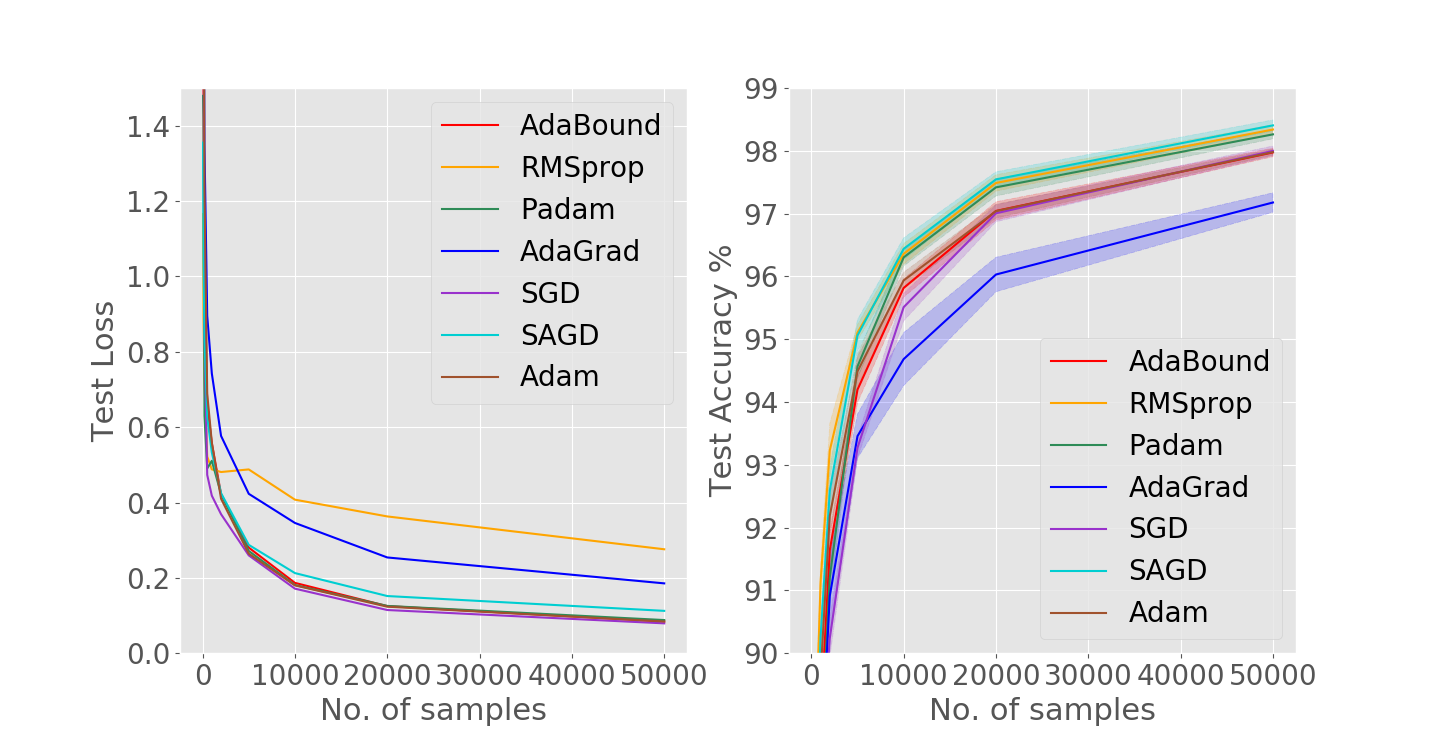
\includegraphics[width = 0.50 \textwidth,trim={2cm 0 2cm 2cm},clip ]{figure/mnist_relu.png}
}\hspace{-0.2in}
\subfigure[MNIST, 2-layer Sigmoid]{
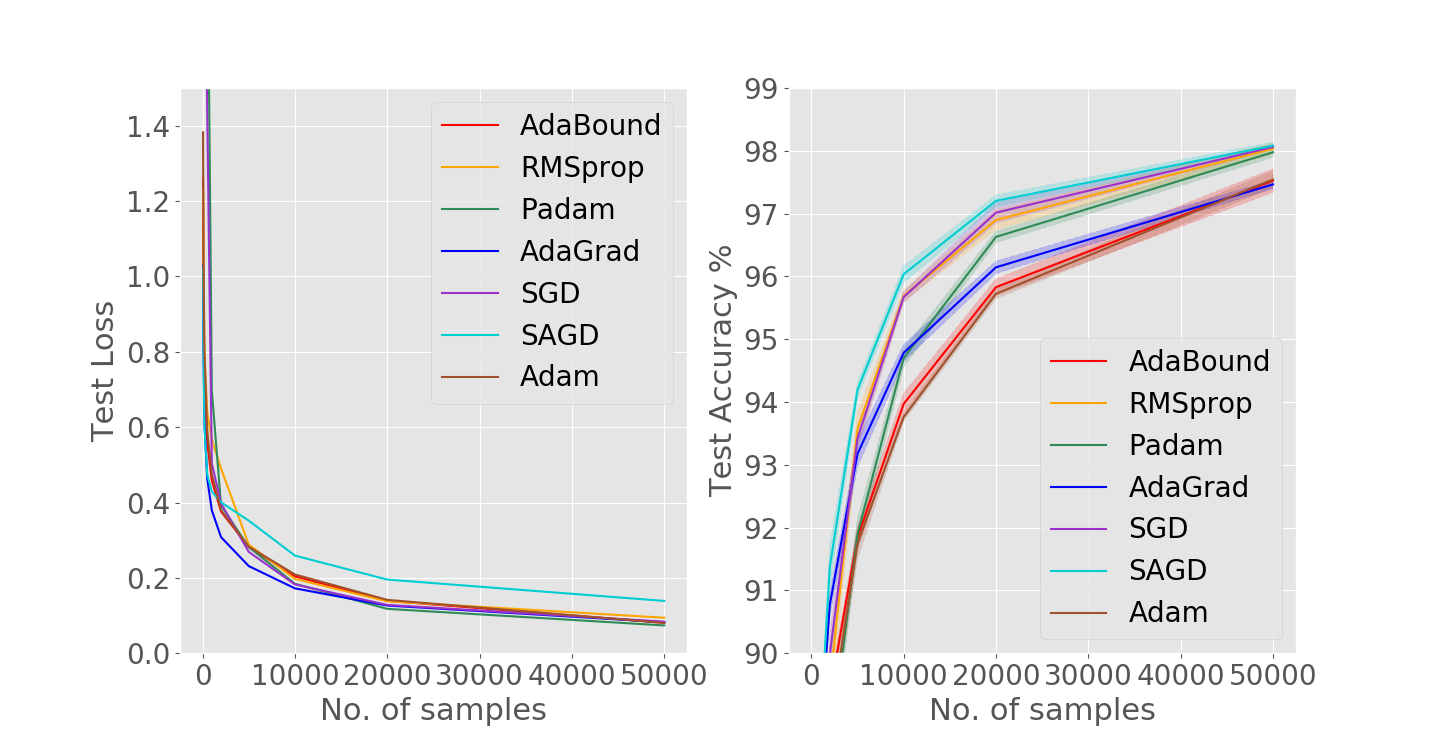
\includegraphics[width = 0.50 \textwidth, trim={2cm 0 2cm 2cm}, clip]{figure/mnist_sigmoid.png}
 }
 }
 \caption[]{Test loss and accuracy of ReLU neural network and Sigmoid neural network on MNIST. The X-axis is the number of train samples, and the Y-axis is the loss/accuracy. In both cases, \textsc{SAGD} obtains the best test accuracy among all the methods.} 
 \label{fig:mnist}
\end{figure*}

\begin{figure*}[t!]
\mbox{
\subfigure[CIFAR10, ResNet-18]{
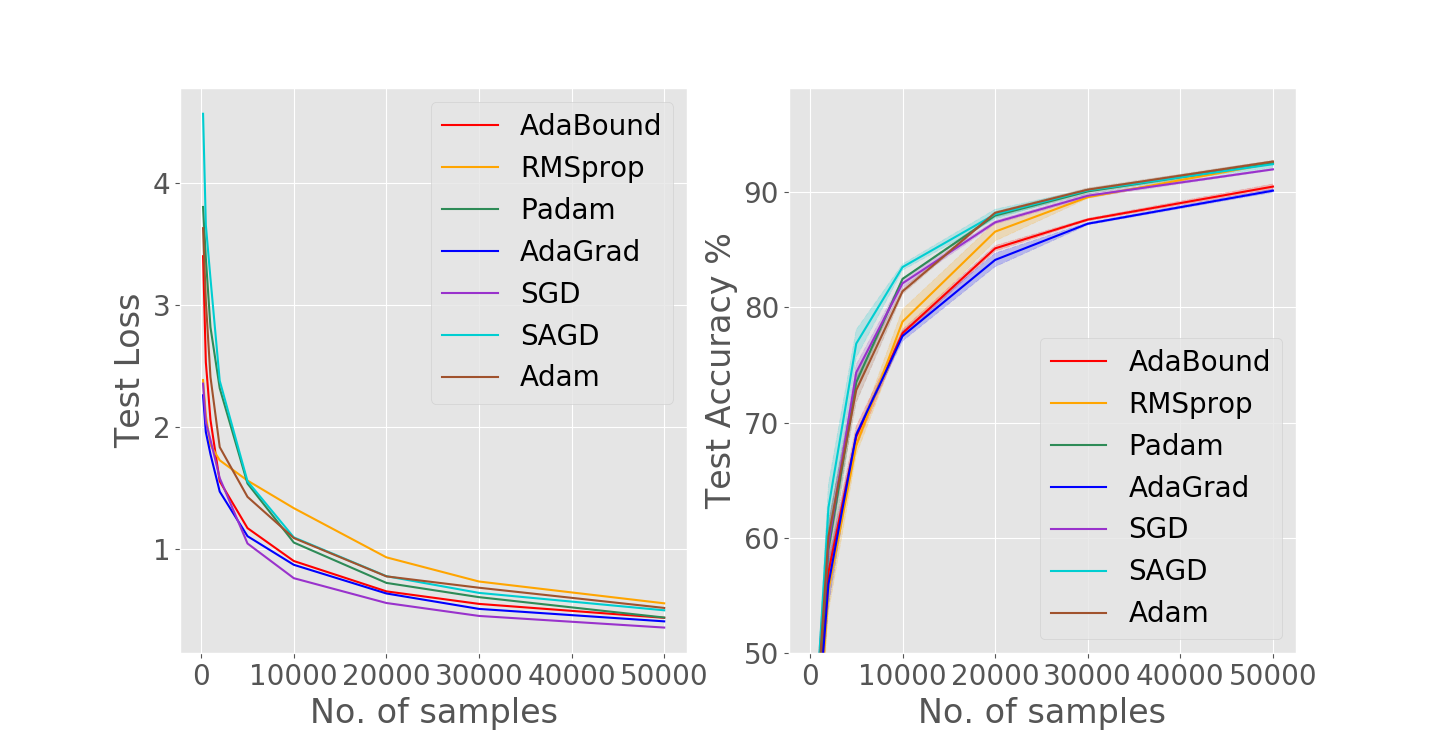
\includegraphics[width = 0.52 \textwidth,trim={2cm 0 2cm 2cm},clip ]{figure/cifar10_resnet.png}
}\hspace{-0.1in}
\subfigure[CIFAR10, VGG-19]{
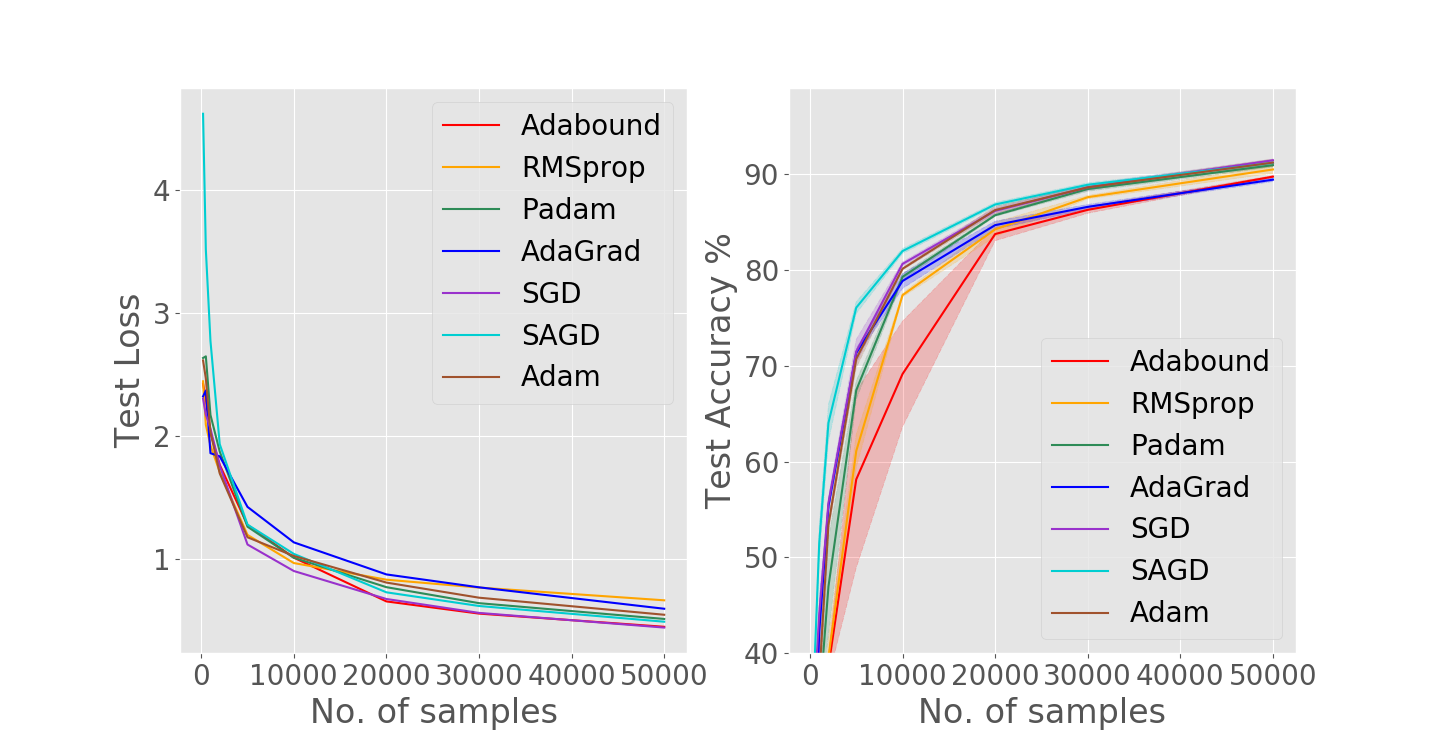
\includegraphics[width = 0.52 \textwidth, trim={2cm 0 2cm 2cm}, clip]{figure/cifar10_vgg.png}
 }
 }
 %\vspace{-0.15in}
 \caption[]{Test loss and accuracy of ResNet-18 andVGG-19 on CIFAR10. The X-axis and the
Y-axis refer to Figure~\ref{fig:mnist}. For ResNet-18, \textsc{SAGD} achieves the lowest test loss. For VGG-19, \textsc{SAGD} achieves the best test accuracy among all the methods. } 
 \label{fig:cifar10}
\end{figure*}

\begin{figure*}[t!]
\mbox{
\subfigure[Penn Treebank, 2-Layer LSTM]{
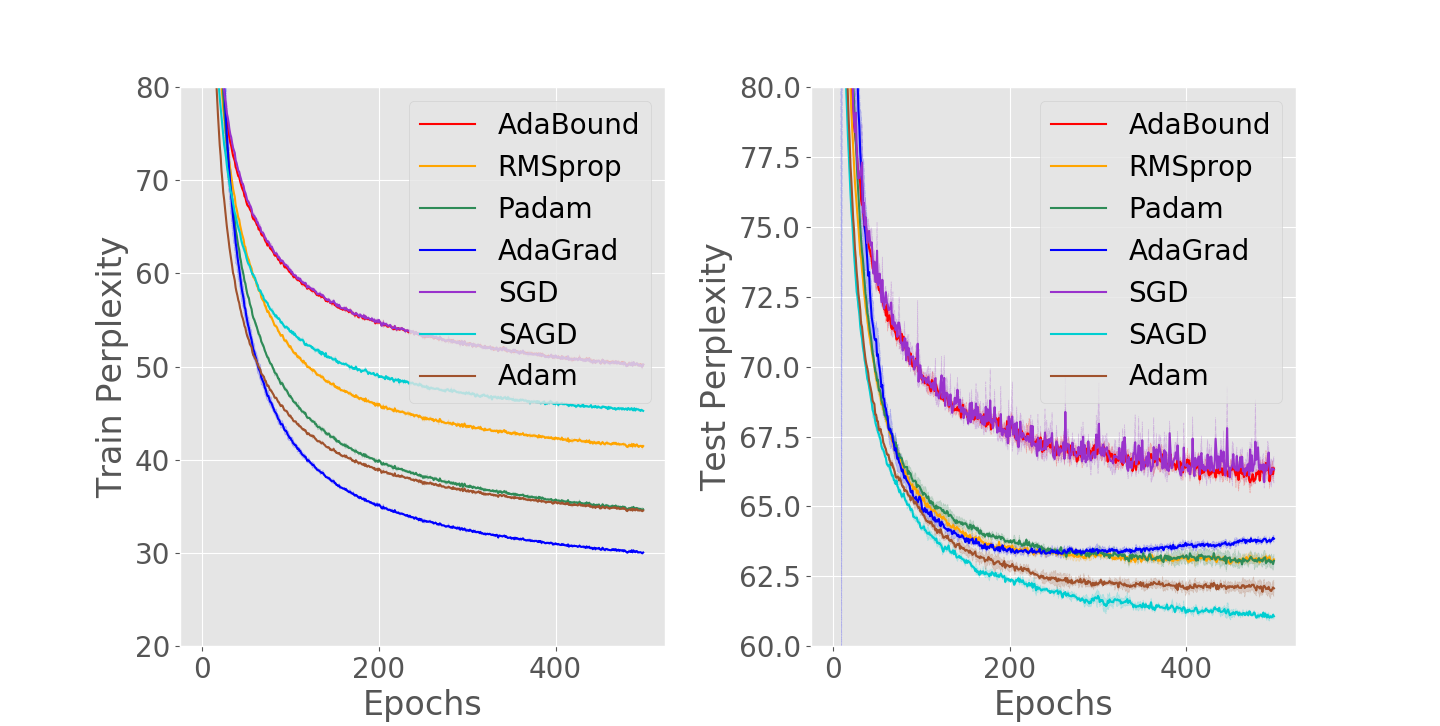
\includegraphics[width = 0.52 \textwidth,trim={2cm 0 2cm 2cm},clip ]{figure/ptb_2lstm.png}
}\hspace{-0.1in}
\subfigure[Penn Treebank, 3-Layer LSTM]{
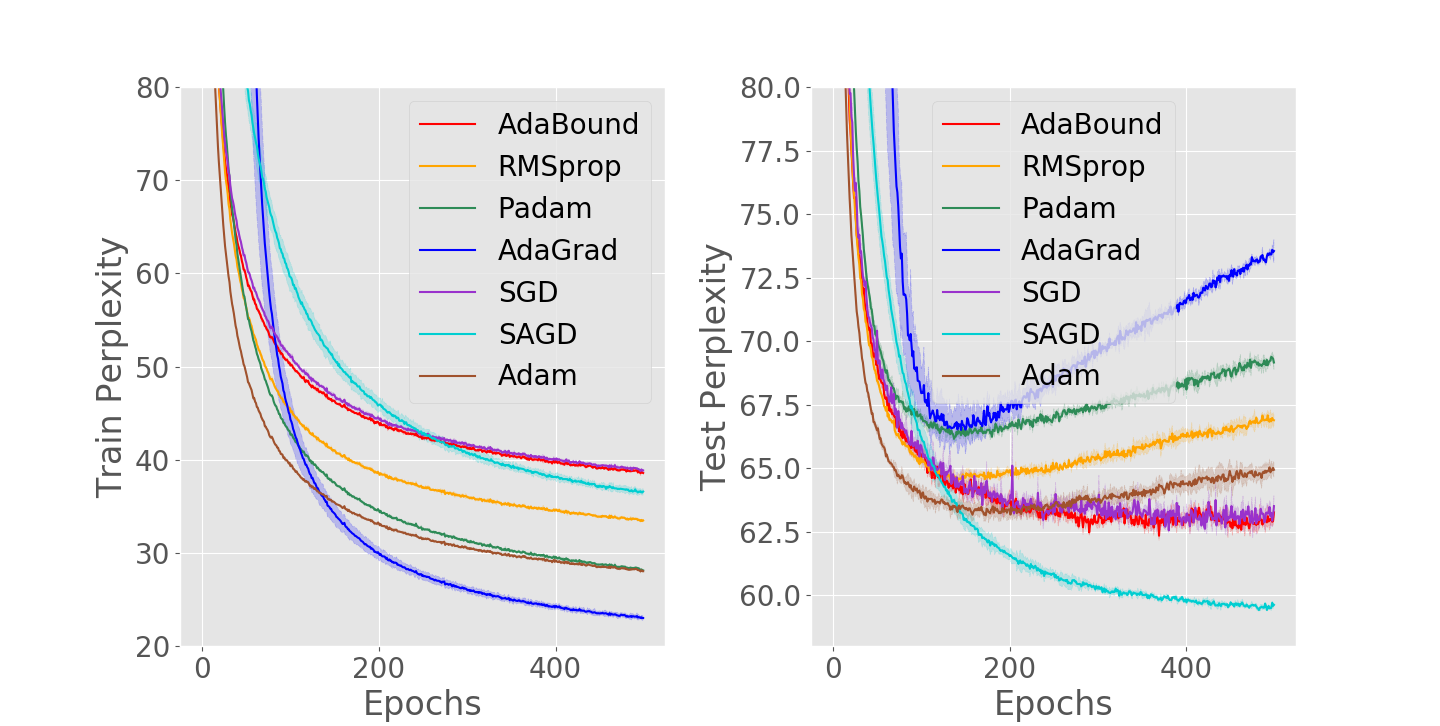
\includegraphics[width = 0.52 \textwidth, trim={2cm 0 2cm 2cm}, clip]{figure/ptb_3lstm.png}
 }
}
\vspace{-0.1in}
 \caption[]{Train and test perplexity of 2-layer LSTM and 3-layer LSTM. The X-axis is the number of epochs, and the Y-axis is the train/test perplexity. Although adaptive methods such as AdGrad, Padam, Adam, and RMsprop achieves better training performance than \textsc{SAGD}, \textsc{SAGD} performs the best in terms of the test perplexity among all the methods.} 
 \label{fig:ptb}
\end{figure*}

%\vspace{-0.05in}
\subsection{Numerical results}\label{subsec:results}
\textbf{Feedforward Neural Network.}
For image classification on MNIST, we focus on two 2-layer fully connected neural networks with ReLU activation and Sigmoid activation, respectively. We run 100 epochs and decay the learning rate by 0.5 every 30 epochs. 
Figure~\ref{fig:mnist} presents the loss and accuracy on the test set given different training sizes. Since all algorithms attain the $100\%$ training accuracy, the performance on the training set is omitted. 
%We can see that for ReLU and Sigmoid neural network, \textsc{SAGD} achieves the best test accuracy
Figure~\ref{fig:mnist} (a) shows that, for ReLU neural network, 
\textsc{SAGD} performs slightly better than the other algorithms in terms of test accuracy. When $n =50000$, \textsc{SAGD} gets a test accuracy of $98.38 \pm 0.13 \%$. 
%The non-adaptive algorithm SGD has a test accuracy of $97.91 \pm 0.21\%$.
%The most recent proposed Padam performs similar to RMSprop
%SGD performs slightly better than adaptive methods in terms of test loss. Regarding the test accuracy, \textsc{SAGD} display slight improvement over the other algorithms. 
Figure~\ref{fig:mnist} (b) presents the results on Sigmoid neural network. \textsc{SAGD} achieves the best test accuracy among all the algorithms. When $n =50000$, \textsc{SAGD} reaches the highest test accuracy of $98.14 \pm 0.11 \%$, outperforming other adaptive algorithms.




\vspace{-0.05in}
\textbf{Convolutional Neural Network.}
We use ResNet-18~\citep{hezh2016} and VGG-19~\citep{sizi2014} for the CIFAR-10 image classification task. We run 100 epochs and decay the learning rate by 0.1 every 30 epochs. 
The results are presented in Figure~\ref{fig:cifar10}. Figure~\ref{fig:cifar10} (a) shows that \textsc{SAGD} has higher test accuracy than the 
other algorithms when the sample size is small i.e., $n \leq 20000$.
When $n = 50000$, \textsc{SAGD} achieves nearly the same test accuracy as Adam, Padam, and RMSprop. In detail, \textsc{SAGD} has test accuracy $92.48 \pm 0.09\%$.
Non-adaptive algorithm 
SGD performs better than the other algorithms in terms of test loss. 
%Regarding the test accuracy, the \textsc{SAGD}, Adam Padam, and SGD perform better than the other.
Figure~\ref{fig:cifar10} (b) reports the results on VGG-19. Although \textsc{SAGD} has a higher test loss than the other algorithms, it achieves the best test accuracy, especially when $n$ is small. Non-adaptive algorithm SGD performs better than the other adaptive gradient algorithms regarding the test accuracy.
When $n= 50000$, SGD has the best test accuracy $91.36 \pm 0.04\%$. \textsc{SAGD} achieves accuracy $91.26 \pm 0.05\%$
%The SGD perform similarly to 
%loss, \textsc{SAGD} perform similarly to SGD. \textsc{SAGD}, SGD and AdaBound achieve the lowest test loss when $n \in [20000, 50000]$. 
%Regarding the test accuracy, we can see that when the training sample size is small, i.e., $n \in [50, 20000]$, \textsc{SAGD} achieves the best test accuracy among all the algorithms. When the sample size is large, i.e, $n \geq 20000$,  \textsc{SAGD}, SGD, and Adam perform better than the other algorithms.

%We use ResNet-18~\citep{hezh2016} and VGG-19~\citep{sizi2014} for the CIFAR-10 image classification task. We run 100 epochs and decay the learning rate by 0.1 every 30 epochs. 

%Results are reported in Figure~\ref{fig:cifar10}. Figure~\ref{fig:cifar10} (a) shows that \textsc{SAGD} and SGD perform better than the other algorithms in terms of the test loss. Regarding the test accuracy, the \textsc{SAGD}, Adam Padam, and SGD outperform the others. Figure~\ref{fig:cifar10} (b) reports the results on VGG-19. In terms of the test loss, \textsc{SAGD} perform similarly to SGD, and the lowest value is attained by \textsc{SAGD}, SGD and AdaBound when $n \in [20000, 50000]$. Regarding the test accuracy, we can see that when the training sample size is small, i.e., $n \in [50, 20000]$, \textsc{SAGD} achieves the best among all the algorithms. When the sample size is large, i.e, $n \geq 20000$,  \textsc{SAGD}, SGD, and Adam perform better than the others.


\begin{table*}[t]
\small
\caption{ Test Perplexity of LSTMs on Penn Treebank. Bold number indicates the best result.}\label{tab:ppl}
	\resizebox{\columnwidth}{!}{%
\begin{tabular}{llllllll}
\toprule[1pt]
 & RMSprop      & Adam         & AdaGrad      & Padam        & AdaBound    & SGD          & \textsc{SAGD}         \\ \hline
2-layer LSTM & 62.87 $\pm$ 0.05 & 60.58 $\pm$ 0.37 & 62.20 $\pm$ 0.29 & 62.85 $\pm$ 0.16 & 65.82 $\pm$0.08 & 65.96 $\pm$ 0.23 & \textbf{61.02 $\pm$ 0.08} \\
3-layer LSTM & 63.97 $\pm$ 018  & 63.23 $\pm$ 004  & 66.25 $\pm$ 0.31 & 66.45 $\pm$ 0.28 & 62.33 $\pm$0.07 & 62.51 $\pm$0.11  & \textbf{59.43 $\pm$ 0.24} \\
\toprule[1pt]
\end{tabular}
}
\end{table*}

\textbf{Recurrent Neural Network.}
Finally, an experiment on Penn Treebank is conducted for the language modeling task with 2-layer Long Short-Term Memory (LSTM)~\citep{stni2018} network and 3-layer LSTM. We train them for a fixed budget of 500 epochs and omit the learning-rate decay. Perplexity is used as the metric to evaluate the performance and learning curves are plotted in Figure~\ref{fig:ptb}. 
Figure~\ref{fig:ptb} (a) shows that for the 2-layer LSTM, AdaGrad, Padam, RMSprop and Adam achieve a lower training perplexity than \textsc{SAGD}. However, \textsc{SAGD} performs the best in terms of the test perplexity. Specifically, \textsc{SAGD} achieves $61.02 \pm 0.08$ test perplexity. 
Especially, It is observed that after 200 epochs, the test perplexity of AdaGrad and Adam starts increasing, but the training perplexity continues decreasing (over-fitting occurs).  
Figure~\ref{fig:ptb} (b) reports the results for the 3-layer LSTM. We can see that the perplexity of AdaGrad, Padam, Adam, and RMSprop start increasing significantly after 150 epochs (\emph{over-fitting}). But the perplexity of \textsc{SAGD} keeps decreasing. \textsc{SAGD} and SGD and AdaBounds perform better than AdaGrad, Padam, Adam, and RMSprop in terms of over-fitting.
Table~\ref{tab:ppl} shows the best test perplexity of 2-layer LSTM and 3-layer LSTM for all the algorithms. We can observe that the \textsc{SAGD} achieves the best test perplexity $59.43 \pm 0.24$ among all the algorithms. 

\section{Conclusion}
\label{sec: conclusion}
In this paper, we focus on the generalization ability of adaptive gradient methods. Concerned with the 
observation that adaptive gradient methods generalize worse than SGD for over-parameterized neural networks and the theoretical understanding of the generalization of those methods is limited,
we propose stable adaptive gradient descent methods (\textsc{SAGD}), which boost the generalization performance in both theory and practice through a novel use of differential privacy. The proposed algorithms generalize well with provable high-probability convergence bounds of the population gradient. Experimental studies demonstrate the proposed algorithms are competitive and often better than baseline algorithms for training deep neural networks. 
In future work, we will consider improving our analysis in several ways, e.g.,  improvement of the dependence on dimension and sharper bounds of \textsc{SAGD} with DPG-Sparse.



\clearpage

\bibliographystyle{abbrvnat}
\bibliography{reference}

\clearpage


\appendix
%\section{Hyperparameter tunning}
%\input{app_setup.tex}

\section{Differential Privacy and Generalization Analysis} \label{sec: pri} \label{sec: pri}



\begin{comment}
\textbf{Assumptions}
\begin{enumerate}
    \item  $ f: \mathbb{R}^d \rightarrow \mathbb{R}$ is differentiable (not necessarily convex), bounded from below by $f^\star$,
and has L-Lipschitz gradient, i.e.,
\begin{equation}
    \nabla f(\w) -\nabla f(\w^\prime) \leq L \|\w-\w^\prime \|, ~ \forall \w, \w^\prime \in \cW
\end{equation}
\item  The noisy gradient is bounded:
\begin{equation}
    \|\tilde \g_t\|_2^2 \leq G
\end{equation}

\item  The $l_1$ norm of the individual gradient is bounded:
\begin{equation}
    \|\nabla \ell (\w,\z) \|_1 \leq G_1, \ \ \  \forall \w \in \cW, \z \in \cZ
\end{equation}
\end{enumerate}


\textbf{Generalization guarantee of differential privacy}




\begin{lemm} \label{lem: gen_basic}
Let $\cA$ be an $\epsilon$-differentially private gradient descent algorithm 
which has access to the training set $S$ of size $n$. Let $\w_t = \cA(S)$ be the parameters generated at each iteration $t \in [T]$ and $\hat \g_t$ be the empircal gradient on $S$. Them, for any $\sigma >0$, $\beta \geq 6\exp(\frac{-\sigma^2 n}{4G_1^2})$, if the privacy cost of $\cA$ satisfies $\epsilon \leq \frac{\sigma}{2G_1}$, we have
\begin{equation}
    \mathbb{P}\left\{ |\hat \g_t^i - \g_t^i| \geq  \sigma \right\} \leq \beta,
\end{equation}
for every $ i\in [d]$ and every $t \in [T]$.
\end{lemm}
\end{comment}



\begin{comment}
\begin{lemm} 
Let $\cA$ be an $(\epsilon, \delta)$-differentially private gradient descent algorithm 
which has access to the training set $S$ of size $n$. Let $\w_t = \cA(S)$ be the parameters generated at each iteration $t \in [T]$ and $\hat \g_t$ be the empircal gradient on $S$. Them, for any $\sigma >0$, $\beta > 0$, if the privacy cost of $\cA$ satisfies $\varepsilon \leq \frac{\sigma}{13}$, $\delta \leq \frac{\sigma \beta}{26 \ln(26/\sigma)}$ and the sample size $n \geq \frac{2\ln(8/\delta)}{\varepsilon^2}$, we have
\begin{equation}
    \mathbb{P}\left\{ |\hat \g_t^i - \g_t^i| \geq  \sigma \right\} \leq \beta,
\end{equation}
for every $ i\in [d]$ and every $t \in [T]$.
\end{lemm}
\end{comment}


%\textbf{Proof of Lemma \ref{lem: gen_adv}:} 



%Note that Lemma \ref{lem: gen_adv} is the instantiation of Corollary 8 from \cite{dwfe15}.


%\subsection{Proof of Lemma \ref{lemma dpp}:} 

%\begin{proof}
%At each iteration $t$, the algorithm is composed of two sequential parts: \textbf{DPG} to access the training set $S$ and compute $\tilde \g_t$, and parameter update based on estimated $\tilde \g_t$. We mark the \textbf{DPG} as part $\mathcal{A}$ and the gradient descent as part $\mathcal{B}$. We first show $\mathcal{A}$ preserves $\frac{G_1}{n\sigma}$-differential privacy. Then according to the \emph{post-processing property} of differential privacy (Proposition 2.1 in \cite{dwro2014}) we have $\mathcal{B} \circ \mathcal{A}$ is also $\frac{G_1}{n\sigma}$-differentially private.
	
%The part $\mathcal{A}$ (DPG-Lap) uses the basic tool from differential privacy, the ``Laplace Mechanism'' (Definition 3.3 in \citep{dwro2014}). 
%The Laplace Mechanism adds i.i.d. Laplace noise to each coordinate of the output. Adding noise from $Lap(\sigma)$ to a query of $G_1/n$
% sensitivity preserves $G_1/n\sigma$-differential privacy by ( Theorem 3.6 in \cite{dwro2014}).
 %Over $T$ iterations, we have $T$ applications of a DPG-Lap. By the advanced composition theorem (Theorem 3.20 in \cite{dwro2014}), $T$ applications of a $\frac{G_1}{n\sigma}$-differentially private algorithm is $(\frac{\sqrt{T \ln(1/\delta)} G_1}{n\sigma}, \delta)$-deferentially private. 
 %So SAGD with DPG-Lap is $(\frac{\sqrt{T \ln(2/\delta)} 2G_1}{n\sigma}, \delta)$-deferentially private.
%\end{proof}




%\subsection{Batch Sparse Vector Mechanism}

%\subsection{Proof of Lemma \ref{lemma: dpp-sparse}:}


By applying Theorem 8 from \citet{dwfe2015a} to gradient computation, we can get the Lemma \ref{lem: gen_adv}.

\lemgenadv*

\proof 
Theorem 8 in \citet{dwfe2015a}  shows that in order to achieve generalization error $\tau$ with probability $1-\rho$ for a $(\epsilon, \delta)$-differentially private algorithm (i.e., in order
to guarantee for every function $\phi_t$, $\forall t \in [T]$, we have $\mathbb{P}\left[\left|\mathcal{P}\left[\phi_t\right]-\mathcal{E}_{S}\left[\phi_t\right]\right| \geq \tau\right] \leq \rho$), where $\mathcal{P}\left[\phi_t\right]$ is the population value, $\mathcal{E}_{S}\left[\phi_t\right]$ is the empirical value evaluated on $S$ and $\rho$ and $\tau$ are any positive constant, we can set the $\epsilon \leq \frac{\tau}{13}$ and $\delta \leq \frac{\tau \rho}{26 \ln (26 / \tau)}$. In our context, $\tau = \sigma$, $\beta =\rho$, $\phi_t$ is 
the gradient computation function $\nabla \ell(\w_t,\z)$,  $\mathcal{P}\left[\phi_t\right]$ represents the population gradient $\g_t^i$, $\forall i\in [p]$, and $\mathcal{E}_{S}\left[\phi_t\right]$ represents the sample gradient $\hat \g_t^i$, $\forall i\in [p]$. Thus we have $\mathbb{P}\left\{\left|\hat{\mathbf{g}}_{t}^{i}-\mathbf{g}_{t}^{i}\right| \geq \tau\right\} \leq \rho$ if $\epsilon \leq \frac{\sigma}{13}, \delta \leq \frac{\sigma \beta}{26 \ln (26 / \sigma)}$.

\subsection{Proof of Lemma \ref{lemma dpp}}


\lemdpp*

\begin{proof}
At each iteration $t$, the algorithm is composed of two sequential parts: DPG to access the training set $S$ and compute $\tilde \g_t$, and parameter update based on estimated $\tilde \g_t$. We mark the DPG as part $\mathcal{A}$ and the gradient descent as part $\mathcal{B}$. We first show $\mathcal{A}$ preserves $\frac{G_1}{n\sigma}$-differential privacy. Then according to the \emph{post-processing property} of differential privacy (Proposition 2.1 in~\cite{dwro2014}) we have $\mathcal{B} \circ \mathcal{A}$ is also $\frac{G_1}{n\sigma}$-differentially private.
	
The part $\mathcal{A}$ (DPG-Lap) uses the basic tool from differential privacy, the ``Laplace Mechanism'' (Definition 3.3 in~\citep{dwro2014}). 
The Laplace Mechanism adds i.i.d. Laplace noise to each coordinate of the output. Adding noise from $Lap(\sigma)$ to a query of $G_1/n$
 sensitivity preserves $G_1/n\sigma$-differential privacy by ( Theorem 3.6 in~\cite{dwro2014}).
 Over $T$ iterations, we have $T$ applications of a DPG-Lap. By the advanced composition theorem (Theorem 3.20 in~\cite{dwro2014}), $T$ applications of a $\frac{G_1}{n\sigma}$-differentially private algorithm is $(\frac{\sqrt{T \ln(1/\delta)} G_1}{n\sigma}, \delta)$-differentially private. 
 So SAGD with DPG-Lap is $(\frac{\sqrt{T \ln(1/\delta)} 2G_1}{n\sigma}, \delta)$-differentially private.
\end{proof}

\subsection{Proof of Theorem \ref{thm: acc_basic}}

\theoaccbasic*

\begin{proof}
The concentration bound is decomposed into two parts:
\begin{equation}
    \begin{split}
    &\mathbb{P} 
    \left\{ \|\tilde \g_t - \g_t\| \geq \sqrt{d}\sigma(1+\mu)\right\} \\
    \leq&   
    \underbrace{ \mathbb{P}\left\{ \|\tilde \g_t - \hat \g_t\| \geq  \sqrt{d}\sigma \mu\right\} }_{\text{$T_1$: empirical error}} 
     + \underbrace{\mathbb{P}\left\{ \|\hat \g_t - \g_t\| \geq \sqrt{d}\sigma \right\}}_{\text{$T_2$: generalization error}} \nr
    \end{split}
\end{equation}
In the above inequality, there are two types of error we need to control. The first type of error, referred to as empirical error $T_1$, is the deviation between the differentially
private estimated gradient $\tilde \g_t$ and the empirical gradient $\hat \g_t$. The second type of error, referred to as generalization error $T_2$, is the deviation
between the empirical gradient $\hat \g_t$ and the population gradient $\g_t$. 

The second term $T_2$ can be bounded thorough the generalization guarantee of differential privacy. Recall that from  Lemma~\ref{lem: gen_adv}, under the condition in Theorem~\ref{thm: acc_sparse}, we have for all $t \in [T]$, $i \in [d]$: 
\begin{equation}
    \mathbb{P}\left\{ |\hat \g_t^i - \g_t^i| \geq  \sigma \right\} \leq \beta \nr
\end{equation}
So that we have 
\begin{equation}\label{eq: gen1}
\mathbb{P}\left\{ \|\hat \g_t - \g_t\| \geq  \sqrt{d}\sigma \right\} \leq \mathbb{P}\left\{ \|\hat \g_t - \g_t\|_\infty \geq  \sigma  \right\} \leq d \mathbb{P}\left\{ |\hat \g_t^i - \g_t^i| \geq  \sigma \right\} \leq d\beta 
\end{equation}

Now we bound the second term $T_1$. Recall that $\tilde \g_t = \hat \g_t + \b_t$, where $\b_t$ is a noise vector with each coordinate drawn from Laplace noise Lap$(\sigma)$. In this case, we have
\begin{align} \label{eq: acc1}
\mathbb{P}\left\{ \|\tilde \g_t - \hat \g_t\| \geq  \sqrt{d}\sigma \mu \right\}  \leq \mathbb{P} \left\{ \|\b_t\| \geq  \sqrt{d}\sigma \mu \right\}  &\leq \mathbb{P} \left\{ \|\b_t\|_\infty \geq  \sigma \mu \right\} \\ 
  &\leq d \mathbb{P} \left\{ |\b_t^i| \geq \sigma \mu \right\}\\
    &= d \exp(-\mu)
\end{align}

The second inequality comes from $\|\b_t\| \leq \sqrt{d}\|\b_t\|_\infty$. The
last equality comes from the property of Laplace distribution. Combine \eqref{eq: gen1} and \eqref{eq: acc1}, we complete the proof.
\end{proof}

\subsection{Proof of Lemma \ref{lemma: dpp-sparse}}

\lemdppsparse*

\begin{proof}
At each iteration $t$, the algorithm is composed of two sequential parts: DPG-Sparse (part $\mathcal{A}$) and parameter update based on estimated $\tilde \g_t$ (part $\mathcal{B}$).
%which accesses the training set $S$ and compute $\tilde \g_t$, and parameter update based on estimated $\tilde \g_t$. We mark the DPG-Sparse as part $\mathcal{A}$ and the gradient descent as part $\mathcal{B}$.
We first show $\mathcal{A}$ preserves $\frac{2G_1}{n\sigma}$-differential privacy. Then according to the \emph{post-processing property} of differential privacy (Proposition 2.1 in~\cite{dwro2014}) we have $\mathcal{B} \circ \mathcal{A}$ is also $\frac{2G_1}{n\sigma}$-differentially private.
	
The part $\mathcal{A}$ (DPG-Sparse) is a composition of basic tools from differential privacy, the ``Sparse Vector Algorithm'' (Algorithm 2 in~\citep{dwro2014}) and the ``Laplace Mechanism'' (Definition 3.3 in~\citep{dwro2014}). In our setting, the sparse vector algorithm takes as input a sequence of $T$ sensitivity $G_1/n$ queries, and for each query, attempts to determine whether the value of the query, evaluated on the private dataset $S_1$, is above a fixed threshold $\gamma + \tau$ or below it. In our instantiation, the  $S_1$ is the private data set, and each function corresponds to the gradient computation function $ \hat \g_t$ which is of sensitivity $G_1/n$. 
%SAGD is equivalent to the following procedure: we run the sparse vector algorithm for with $T$ queries corresponding to  gradient computation function $ \hat \g_t, t \in [T]$, and noise rate $\sigma$. 
By the privacy guarantee of the sparse vector algorithm, the sparse vector portion of SAGD satisfies $G_1/n\sigma$-differential privacy. The Laplace mechanism portion of SAGD
satisfies $G_1/n\sigma$-differential privacy by ( Theorem 3.6 in~\cite{dwro2014}). Finally, the composition of two mechanisms satisfies $\frac{2G_1}{n\sigma}$-differential privacy. For the sparse vector technique, only the query that fails the validation, corresponding to the `above threshold', release the privacy
of private dataset $S_1$ and pays a $\frac{2G_1}{n\sigma}$ privacy cost. 
Over all the iterations $T$, We have $C_{s}$ queries fail the validation.
Thus, by the advanced composition theorem (Theorem 3.20 in~\cite{dwro2014}), $C_{s}$ applications of a $\frac{2G}{n\sigma}$-differentially private algorithm is  $(\frac{\sqrt{C_{s} \ln(2/\delta)} 2G_1}{n\sigma}, \delta)$-differentially private. So SAGD with DPG-Sparse is $(\frac{\sqrt{C_{s} \ln(2/\delta)} 2G_1}{n\sigma}, \delta)$-differentially private.
\end{proof}
    


\subsection{Proof of Theorem \ref{thm: acc_sparse}:}

\theoaccsparse*

\begin{proof}
The concentration bound can be decomposed into two parts:
\begin{align}\notag
\mathbb{P}\left\{ \|\tilde \g_t - \g_t\| \geq \sqrt{d}\sigma(1+\mu)\right\}  \leq \underbrace{ \mathbb{P}\left\{ \|\tilde \g_t - \hat \g_{s_1,t}\| \geq \sqrt{d}\sigma \mu\right\} }_{\text{$T_1$: empirical error}} +  \underbrace{\mathbb{P}\left\{ \|\hat \g_{s_1,t} - \g_t\| \geq \sqrt{d}\sigma \right\}}_{\text{$T_2$: generalization error}}
\end{align}
%In the above inequality, there are two types of error we need to control. The first type of error, referred to as empirical error $T_1$, is the the deviation between the differentially
%private estimate gradient $\tilde \g_t$ and the empirical gradient $\hat \g_t$. The second type of error, referred to as generalization error $T_2$, is the deviation
%between the empirical gradient $\hat \g_t$ and the population gradient $\g_t$. 

%The second term $T_2$ can be bounded thorough the generalization guarantee of differential privacy. Recall that from  Lemma \ref{lem: gen_adv}, under the condition in Theorem \ref{thm: acc_sparse}, we have for all $t \in [T]$ and for all $i \in [d]$: 
%\begin{equation}
%    \mathbb{P}\left\{ |\hat \g_{s_1,t}^i - \g_t^i| \geq  \sigma \right\} \leq \beta
%\end{equation}
So that we have 
\begin{align} \notag
    \mathbb{P}\left\{ \|\hat \g_{s_1,t} - \g_t\| \geq  \sqrt{d}\sigma \right\} 
    &\leq \mathbb{P}\left\{ \|\hat \g_{s_1,t} - \g_t\|_\infty \geq  \sigma \right\} \\\notag
    &\leq d \mathbb{P}\left\{ |\hat \g_{s_1,t}^i - \g_t^i| \geq  \sigma \right\} \\\label{eq: gen2}
    &\leq d\beta 
\end{align}

Now we bound the second term $T_1$ by considering two cases, by depending on whether DPG-3 answers the query $\tilde \g_t$ by 
returning $\tilde \g_t = \hat \g_{s_1,t} + \v_t$ or by returning $\tilde \g_t = \hat \g_{s_2,t}$. In the first case, we have 
\begin{equation}
    \|\tilde \g_t - \hat \g_{s_1,t}\| = \|\v_t\| \nr
\end{equation}
and
\begin{equation}
\begin{split}
    \mathbb{P}\left\{ \|\tilde \g_t - \hat \g_{s_1,t}\| \geq \sqrt{d}\sigma \mu  \right\}  = \mathbb{P} \left\{ \|\v_t\| \geq  \sqrt{d}\sigma \mu \right\} \leq d \exp(-\mu) \nr
\end{split}
\end{equation}
The last inequality comes from the $\|\v_t\| \leq \sqrt{d}\|\v_t\|_\infty$ and properties of the Laplace distribution. 

In the second case, we have 
\begin{equation}
    \|\tilde \g_t - \hat \g_{s_1,t} \| = \| \hat \g_{s_2,t} -\hat \g_{s_1,t} \| \leq |\gamma| + |\tau| \nr
\end{equation}
and 
\begin{equation}
\begin{split}
\mathbb{P} \left\{ \|\tilde \g_t - \hat \g_{s_1,t}\| \geq \sqrt{d}\sigma \mu  \right\} =& \mathbb{P} \left\{ |\gamma| + |\tau| 
 \geq   \sqrt{d}\sigma \mu \right\} \\ 
 \leq&
  \mathbb{P} \left\{ |\gamma|  \geq   \frac{2}{6}\sqrt{d}\sigma \mu \right\} +  \mathbb{P} \left\{ |\tau|  \geq   \frac{4}{6}\sqrt{d}\sigma \mu \right\} \\
 =& 2\exp(-\sqrt{d}\mu /6) \nr
\end{split}
\end{equation}

Combining these two cases, we have
\begin{align}\notag 
\mathbb{P} 
\left\{ \|\tilde \g_t - \hat \g_{s_1,t}\| \geq \sqrt{d}\sigma \mu  \right\}  \leq & \max \left\{ 
\mathbb{P} \left\{ \|\v_t\| \geq  \sqrt{d}\sigma \mu \right\}, 
\mathbb{P} \left\{ |\gamma| + |\tau|
 \geq   \sqrt{d}\sigma \mu \right\}
\right\} \\\notag 
\leq& \max \left\{ d\exp(-\mu), 2\exp(-\sqrt{d}\mu /6) \right\} \\\label{eq: acc2}
=& d\exp(-\mu)
\end{align}

Combine \eqref{eq: gen2} and \eqref{eq: acc2}, we complete the proof.

\end{proof}


\clearpage
\section{Non-asymptotic Convergence analysis}
%\section{CONVERGENCE ANALYSIS}

In this section, we present the proof of Theorem \ref{thm: main_rmsprop}, \ref{thm: main_rmsprop_sparse}
\label{sec: thm2_proof}, \ref{thm: main_rmsprop_mini}.

\subsection{Proof of Theorem \ref{thm: main_rmsprop} and Theorem \ref{thm: main_rmsprop_sparse}}

The proof of Theorem \ref{thm: main_rmsprop} consists of two parts: We first prove that the convergence rate of a gradient-based iterative algorithm is related to the gradient concentration error $\alpha$ and its iteration 
time $T$. Then we combine the concentration error $\alpha$ achieved by SAGD with DPG-Lap in Theorem \ref{thm: acc_basic} with the first part to complete the proof of Theorem \ref{thm: main_rmsprop}. 
To simplify the analysis, we first use $\alpha$ and $\xi$ to denote the generalization error $\sqrt{d} \sigma(1+\mu)$ and probability $d \beta+d \exp (-\mu)$ in Theorem \ref{thm: acc_basic} in the following analysis. The details are presented in the following theorem.
\begin{theo} \label{thm: simp_gen}
Let $\tilde \g_1,...,\tilde \g_T$ be the noisy gradients generated in Algorithm 1 through DPG oracle over $T$ iterations.
Then, for every $t \in [T]$, $\tilde \g_t$ satisfies
%Let $\g_t = \nabla f(\w_t)$ be the population gradient at parameter $w_t$. For $t \in [T]$, the noisy gradient $\tilde \g_t$ from DPG with oracle satisfies
\begin{equation} \nr
    \mathbb{P}\{\|\tilde \g_t - \g_t\| \geq \alpha \} \leq \xi \, ,
\end{equation}
where the values of $\alpha$ and $\xi$ are given in Section \ref{sec: pri}. 
\end{theo}
With the guarantee of Theorem \ref{thm: simp_gen}, we have the following theorem showing the convergence of SAGD.
\begin{theo} \label{thm: opt_rmsprop}
 let $\eta_t = \eta$. Further more assume that $\nu$, $\beta$ and $\eta$ are chosen such that the following conditions satisfied: $\eta \leq \frac{\nu}{2L}$. 
 Under the Assumption A1 and A2, the Algorithm 1 with $T$ iterations, $\phi_t(\tilde \g_1,...,\tilde \g_t) = \tilde \g_t$ and $ \v_t = \left(1-\beta_{2}\right) \sum_{i=1}^{t} \beta_{2}^{t-i} \tilde \g_{i}^{2}$ achieves:
\begin{equation}\label{eq: opt_rmsprop}
 \min_{t = 1,..., T}\|\nabla f(x_t)\|^2 \leq
    \left(G+\nu \right) \times \left(   \frac{ f(\w_1) - f^\star}{\eta T} + \frac{3 \alpha^2}{4\nu}\right) \, ,
\end{equation}
with probability at least $1-T\xi$.
\end{theo}
We can now tackle the proof of our result stated in Theorem \ref{thm: opt_rmsprop}.
\begin{proof}
Using the update rule of RMSprop, we have $\phi_t(\tilde \g_1,...,\tilde \g_t) = \tilde \g_t$ and $ \psi_t(\tilde \g_1,...,\tilde \g_t) = \left(1-\beta_{2}\right) \sum_{i=1}^{t} \beta_{2}^{t-i} \tilde \g_{i}^{2}$.
Thus, we can rewrite the update of Algorithm \ref{algo: StAda} as:
\begin{equation}
\begin{split} \nr
    \w_{t+1} = \w_t - \eta_t \tilde  \g_t /(\sqrt{\v_t} + \nu) \ \ \text{and} \ \  \v_t = \left(1-\beta_{2}\right) \sum_{i=1}^{t} \beta_{2}^{t-i} \tilde \g_{i}^{2} \, .
\end{split}
\end{equation}
Let $\Delta_t = \tilde \g_t - g_t$, we obtain:
\begin{equation} \notag
\begin{split}
 & f (\w_{t+1}) \\
\leq & f(\w_t) + \left<\g_t, \w_{t+1}-\w_t\right> + \frac{L}{2} \left\|\w_{t+1}-\w_t \right\|^2\\ 
=& f(\w_t) -\eta_t \left<\g_t, \tilde \g_t/(\sqrt{\v_t} +\nu) \right> + \frac{L\eta_t^2}{2} \left\|\frac{\tilde \g_t}{(\sqrt{\v_t} +\nu)} \right\|^2\\ 
=& f(\w_t) -\eta_t \left<\g_t, \frac{\g_t +\Delta_t}{\sqrt{\v_t} +\nu} \right> + \frac{L\eta_t^2}{2}\left\|\frac{\g_t + \Delta_t}{\sqrt{\v_t} +\nu}\right\|^2 \\ 
\leq& f(\w_t) -\eta_t \left<\g_t, \frac{\g_t }{\sqrt{\v_t} +\nu}\right> -\eta_t \left<\g_t, \frac{\Delta_t }{\sqrt{\v_t} +\nu} \right> + L\eta_t^2\left(\left\|\frac{\g_t }{\sqrt{\v_t} +\nu}\right\|^2 + \left\|\frac{ \Delta_t}{\sqrt{\v_t} +\nu}\right\|^2   \right) \\ 
  =& f(\w_t) -\eta_t \sum_{i=1}^d \frac{\left[\g_t\right]_i^2}{\sqrt{\v_t^i} +\nu} - \eta_t \sum_{i=1}^d \frac{\g_t^i \Delta_t^i}{\sqrt{\v_t^i} +\nu} +  L\eta_t^2\left(\sum_{i=1}^d\frac{[\g_t]_i^2 }{(\sqrt{\v_t^i} +\nu)^2} + \sum_{i=1}^d\frac{[\Delta_t]_i^2 }{(\sqrt{\v_t^i} +\nu)^2} 
    \right) \\ 
 \leq& f(\w_t) -\eta_t \sum_{i=1}^d \frac{[\g_t]_i^2}{\sqrt{\v_t^i} +\nu}  + \frac{\eta_t}{2}\sum_{i=1}^d \frac{[\g_t]_i^2 + [\Delta_t]_i^2}{\sqrt{\v_t^i} +  +\nu}  + \frac{L\eta_t^2}{\nu}\left(\sum_{i=1}^d\frac{[\g_t]_i^2 }{\sqrt{\v_t^i} +\nu} + \sum_{i=1}^d\frac{[\Delta_t]_i^2 }{\sqrt{\v_t^i} +\nu}
    \right) \\ 
 = & f(\w_t) - \left(\eta_t -\frac{\eta_t}{2} - \frac{L\eta_t^2}{\nu} \right)\sum_{i=1}^d\frac{[\g_t]_i^2 }{\sqrt{\v_t^i} +\nu}  +\left(  \frac{\eta_t}{2} + \frac{L\eta_t^2}{\nu} \right)\sum_{i=1}^d\frac{[\Delta_t]_i^2 }{\sqrt{\v_t^i} +\nu}    \,.
 \end{split}
\end{equation}


Given the parameter setting from the theorem, we see the following condition hold:
\begin{equation} \nr
    \frac{L\eta_t}{\nu} \leq \frac{1}{4}.
\end{equation}
Then we obtain
\begin{align} 
\nr f(\w_{t+1})& \leq f(\w_t) - \frac{\eta}{4} \sum_{i=1}^{d} \frac{\left[\mathbf{g}_{t}\right]_{i}^{2}}{\sqrt{\mathbf{v}_{t}^{i}}+\nu}+\frac{3 \eta}{4} \sum_{i=1}^{d} \frac{\left[\Delta_{t}\right]_{i}^{2}}{\sqrt{\v_t^i} + \nu} \\ 
& \leq f(\w_t) - \frac{\eta}{G + \nu} \|\g_t\|^2 + \frac{3\eta}{4\epsilon} \|\Delta_t\|^2 \nr  \, .
\end{align}
The second inequality follows from the fact that $0 \leq \v_t^i \leq G^2$. Using the telescoping sum and rearranging the inequality,  we obtain
\begin{align} \nr
\frac{\eta}{G + \nu} \sum_{t=1}^T \|\g_t\|^2  \leq f(\w_1) - f^\star + \frac{3\eta}{4\epsilon} \sum_{t=1}^T  \|\Delta_t\|^2  \, .
\end{align}

Multiplying with $\frac{G +\nu}{\eta T}$ on both sides and with the guarantee in Theorem 1 that $\|\Delta_t\| \leq \alpha$ with probability at least $1-\xi$,  we obtain 
\begin{equation} \nr
\min_{t = 1,..., T}\|\g_t\|^2 \leq \left(G+\nu \right) \times \left(   \frac{ f(\w_1) - f^\star}{\eta T} + \frac{3 \alpha^2}{4\nu}\right)  \, ,
\end{equation}
with probability at least $1-T\xi$.\\


\end{proof}

\vspace{0.1in}

We may now present the proof of our Theorem \ref{thm: main_rmsprop}.
\theomainrmsprop*
\begin{proof}
First consider the gradient concentration bound achieved by SAGD (Theorem \ref{thm: acc_basic} and Theorem \ref{thm: acc_sparse}) that if $ \frac{2n\sigma^2}{G_1^2}\leq T \leq \frac{n^2 \sigma^4}{169 \ln(1/(\sigma \beta))G_1^2}$, we have 
\begin{equation}
\begin{split}
\mathbb{P}\left\{\|\tilde \g_t - \g_t\| \geq \sqrt{d}\sigma(1+\mu)\right\} \leq d\beta + d\exp(-\mu), \ \ \forall t \in [T].
\end{split} \nr
\end{equation}
Then bring the setting in Theorem \ref{thm: main_rmsprop} that $\sigma = 1/n^{1/3}$, let $\mu = \ln (1/\beta)$ and $\beta = 1/(d n^{5/3})$, we have
\begin{equation}
 \|\tilde \g_t - \g_t\|^2 \leq d(1+\ln d + \frac{5}{3}\ln n)^2/n^{2/3}    \nr  \, ,
\end{equation}
with probability at least $1- 1/n^{5/3}$, when we set $T = n^{2/3}/\left(169G_1^2(\ln d + \frac{7}{3}\ln n)\right)$. 

Connect this result with Theorem \ref{thm: opt_rmsprop}, so that we have $\alpha^2 = d(1+\ln d + \frac{5}{3}\ln n)^2/n^{2/3}$ and $\xi = 1/n^{5/3}$. Bring the value $\alpha^2$, $\xi$ and $T = n^{2/3}/\left(169G_1^2(\ln d + \frac{7}{3}\ln n)\right)$ into \eqref{eq: opt_rmsprop}, with $\rho_{n,d} = O \left(\ln n + \ln d \right)$, we have
\begin{align*}
\min_{t = 1,..., T}\|\nabla f(\w_t)\|^2 \leq O\left( \frac{\rho_{n,d} \left(f(\w_1) - f^\star \right)}{n^{2/3}} \right) + O \left( \frac{d \rho_{n,d}^2}{n^{2/3}}\right)\, ,
\end{align*}
with probability at least $1-O\left(\frac{1}{\rho_{n,d} n}\right)$ which concludes the proof.
\end{proof}


\theormspropsparse*


\begin{proof}
The proof of Theorem \ref{thm: main_rmsprop_sparse} follows the proof of Theorem \ref{thm: main_rmsprop} by considering the case $C_{s} = T$.
\end{proof}


\subsection{Proof of Theorem \ref{thm: main_rmsprop_mini}} 

\theomini*

\begin{proof} When mini-batch SAGD calls \textbf{DPG} to access each batch $s_k$ with size $m$ for $T$ times, we have mini-batch SAGD preserves $(\frac{\sqrt{T \ln(1/\delta)} G_1}{m\sigma}, \delta)$-deferential privacy for each batch $s_k$. Now consider the gradient concentration bound achieved by DPG-Lap (Theorem \ref{thm: acc_basic}) that if $ \frac{2m\sigma^2}{G_1^2}\leq T \leq \frac{m^2 \sigma^4}{169 \ln(1/(\sigma \beta))G_1^2}$, we have 
\begin{align*}
\mathbb{P}\left\{\|\tilde \g_t - \g_t\| \geq \sqrt{d}\sigma(1+\mu)\right\} \leq d\beta + d\exp(-\mu), \ \ \forall t \in [T]  \, .
\end{align*}
Then bring the setting in Theorem \ref{thm: main_rmsprop_mini} that $\sigma = 1/(nm)^{1/6}$, let $\mu = \ln (1/\beta)$ and $\beta = 1/(d n^{5/3})$, we have
\begin{equation}
 \|\tilde \g_t - \g_t\|^2 \leq d(1+\ln d + \frac{5}{3}\ln n)^2/n^{2/3}   \nr  \, ,
\end{equation}
with probability at least $1- 1/n^{5/3}$, when we set $T = (mn)^{1/3}/\left(169G_1^2(\ln d + \frac{7}{3}\ln n)\right)$. 


Connect this result with Theorem \ref{thm: opt_rmsprop}, so that we have $\alpha^2 = d(1+\ln d + \frac{5}{3}\ln n)^2/(mn)^{1/3}$ and $\xi = 1/n^{5/3}$. Bring the value $\alpha^2$, $\xi$ and $T = (mn)^{1/3}/\left(169G_1^2(\ln d + \frac{7}{3}\ln n)\right)$ into \eqref{eq: opt_rmsprop}, with $\rho_{n,d} = O \left(\ln n + \ln d \right)$, we have
\begin{align*}
\min_{t = 1,..., T}\|\nabla f(\w_t)\|^2 \leq O\left( \frac{\rho_{n,d} \left(f(\w_1) - f^\star \right)}{(mn)^{1/3}} \right) + O \left( \frac{d \rho_{n,d}^2}{(mn)^{1/3}}\right)  \, ,
\end{align*} 
with probability at least $1-O\left(\frac{1}{\rho_{n,d} n}\right)$. Here we complete the proof.

\end{proof}




%\section{Convergence Analysis of SAGD with the Update Rule of SGD, AdaGrad-Norm and AdaGrad}
%\input{app_opt_analysis.tex}

%\section{Main Theorems}
%\label{sec: main_thm}
%\input{app_main_thm.tex}

%-----------------------------------------------------------------------------
%\vspace{0.4cm}

\end{document} 
